\documentclass[a4j,12pt]{jreport}
\usepackage[dvipdfmx]{color}
\usepackage{color}
%\usepackage[dvips]{graphicx}
%\usepackage{multicol}
\usepackage{amsmath, ascmac, amssymb}
\usepackage{borderhead}
\usepackage[dvipdfmx]{graphicx}
\usepackage{graphicx}
\usepackage{subfigure}
\usepackage{multicol}
\usepackage{color}
\usepackage[dvipdfmx,breaklinks=true,a4paper=true,colorlinks,
linkcolor=black,citecolor=black,urlcolor=black]{hyperref}
\usepackage[dvipdfmx]{pxjahyper}
\usepackage{here}
\newcommand{\figref}[1]{\textgt{図 \ref{#1}}}
\newcommand{\tableref}[1]{\textgt{表 \ref{#1}}}
\newcommand{\chapterref}[1]{\textgt{第 \ref{#1} 章}}

\newcommand{\parfrac}[2]{\frac{\partial #1}{\partial #2}}
%\documentclass[a4j,12pt]{jarticle}
%%%%%行間の幅を再定義
\renewcommand{\baselinestretch}{1.15}
\renewcommand{\bibname}{参考文献}
%%%%%sectionで番号をつける深さ
%\setcounter{secnumdepth}{2}
%%%%%目次に書き出す深さ
\setcounter{tocdepth}{3}
\setcounter{secnumdepth}{3}
\setlength{\footskip}{7mm}
%%%%%%%%%%表紙
\begin{titlepage}
\vspace{-8cm}

\title{
	平成30年度 修士研究論文\vspace{1cm}\\
	\huge  レスキュー犬の一人称動画\\を用いた動作分類\vspace{6cm}
}

\author{
	電気通信大学大学院 情報理工学研究科\\
	情報学専攻 メディア情報学プログラム\\
	1730010\hspace{1cm}荒木 勇人\\
	主任指導教員 柳井 啓司 教授\\
        指導教員 橋本 直己 准教授
}

\date{
平成31年1月28日
}
\end{titlepage}



%%%%%%%%%%%%%%%%%%%%本文
\begin{document}

%%%%%%%%%%表紙
\maketitle
\thispagestyle{empty}
\pagebreak

\begin{abstract}

被災地での災害救助を補助する犬をレスキュー(災害救助)犬といい,カメラなどの計測装置を装備したレスキュー犬をサイバーレスキュー犬と言う.本研究では,犬にとりつけたセンサからサイバーレスキュー犬の活動をした.
光学センサと音声センサから得られた映像および音声データを含む動画像とCNNを用いて動作毎に分類するsound/image-based three-stream CNNの提案と,提案手法をマルチクラス推定に用いた実験を行なった.
光学センサから得られた情報は犬の一人称視点の映像である.これは通常,分類の対象とされる三人称視点の映像とは大きく異なる.
第三者視点映像は基本的に背景が動かず,前景となる被写体の動きを捉える.対して一人称視点映像は,センサそのものが動き回り,背景や前景が存在しない.
被写体の識別が主なアプローチとなる第三者視点映像の認識よりも,一人称視点映像の認識の難易度は高いと言える.
sound/image-based three-stream CNNは動画から得られた静止画像・optical flow画像・音声を入力とする動画識別ネットワークである.
本提案手法の有効性を示すため,3つの入力それぞれ単体とその組み合わせパターン
(静止画像単体,optical flow画像単体,音声単体,静止画像+optical flow画像,静止画像+音声,optical flow画像+音声)
を用いた識別との比較実験を行なった.
結果は,51.8\%で提案手法で最も高い精度が得られた.
推定には,レスキュー犬の訓練の様子を撮影したデータセットを用いた.このデータセットは現在も作成中であり,まだ学習のデータ量が十分とは言えない.
一人称視点動画からのマルチクラス推定というタスクと,レスキュー犬訓練データセットの複雑さのあいまったチャレンジングなタスクであることを踏まえると,本研究では次に繋がる十分な結果が得られたと言える.


\par


\end{abstract}

%%%%%%%%%%目次
%\pagestyle{plain}
\pagestyle{jgraduate}

\pagenumbering{roman}

\tableofcontents

\pagebreak

\pagenumbering{arabic}
\newpage

%%%%%%%%%%%%%%%%%%%%%%%%%%%%%%%%%%%%%%%%%%%%%%%%%%%%
%%%%%%%%%% 1章
\chapter{はじめに}
被災地での救助活動を行う際に,訓練されたレスキュー犬(災害救助犬)が人間の補助として探査を行う場合がある~(図~\ref{resque}).
災害救助犬を育成し、現場に派遣する団体は日本国内に複数存在し,必要に応じて現場に派遣される.
レスキュー犬は,犬としての特性を生かして人間と協力して被災地の探索を行う.
レスキュー犬にはがれきの隙間などの狭い空間,倒壊した建築物など人間には踏破困難な環境でも探査可能であったり,またその発達した嗅覚を頼りにした探査が可能である.このように,人間では探査が困難あるいは不可能な環境においても人間の能力をレスキュー犬が補うことで効果的な救助活動が期待される.
しかし,彼らレスキュー犬は人間に向けた言語を持たない.そのため,人間はレスキュー犬の行動をよく観察し,彼らが収集した情報を彼らの様子から推察,理解しなくてはならない.
現状では,レスキュー犬を直接指揮するハンドラーと呼ばれる人間がレスキュー犬の行動を手動でマーキングして犬の周辺環境の情報収集と理解に努めている.
収集された情報は消防などのハンドラーらを統括する指揮命令者に口頭伝達され,現場の把握に活かされる.
このレスキュー犬と人間との共同探索の問題点として,トリアージ(緊急度に従った手当の優先順位付け)のための災害現場周辺環境情報や,要救助者情報の不足があげられる.
また,ハンドラーによる記録はどうしても主観的になるので客観性に欠け,さらにそれが口頭伝達されることで正確性がより欠落する.
レスキュー犬によって収集された情報を個人の主観に基づくことなく分類し,整理された情報を共有できれば災害救助活動の効率化がより期待される.

本研究では,レスキュー犬にセンサを装着して得られた一人称動画を用いてレスキュー犬の行動を分類すること目的とする.
本研究では最初に深層学習を用いた画像認識手法を,一人称映像から抽出した静止画像に適用して動作分類を行う予備実験を行った.
この予備実験で犬一人称視点映像からの動作分類タスクに対してCNNを用いた推定が有効であることを確認した.
予備実験を踏まえて,CNNを利用し,静止画像に加えて一人称画像から抽出した動き情報と音声情報を利用したマルチモーダルなレスキュー犬行動推定を行った.
本研究により,レスキュー犬が今何をしているのかハンドラーが目視できない場合でも機械的に判断することが可能となり,トリアージに必要な情報が整理され,災害救助活動の効率化が期待される.
\begin{figure}[htbp]
 \begin{center}
  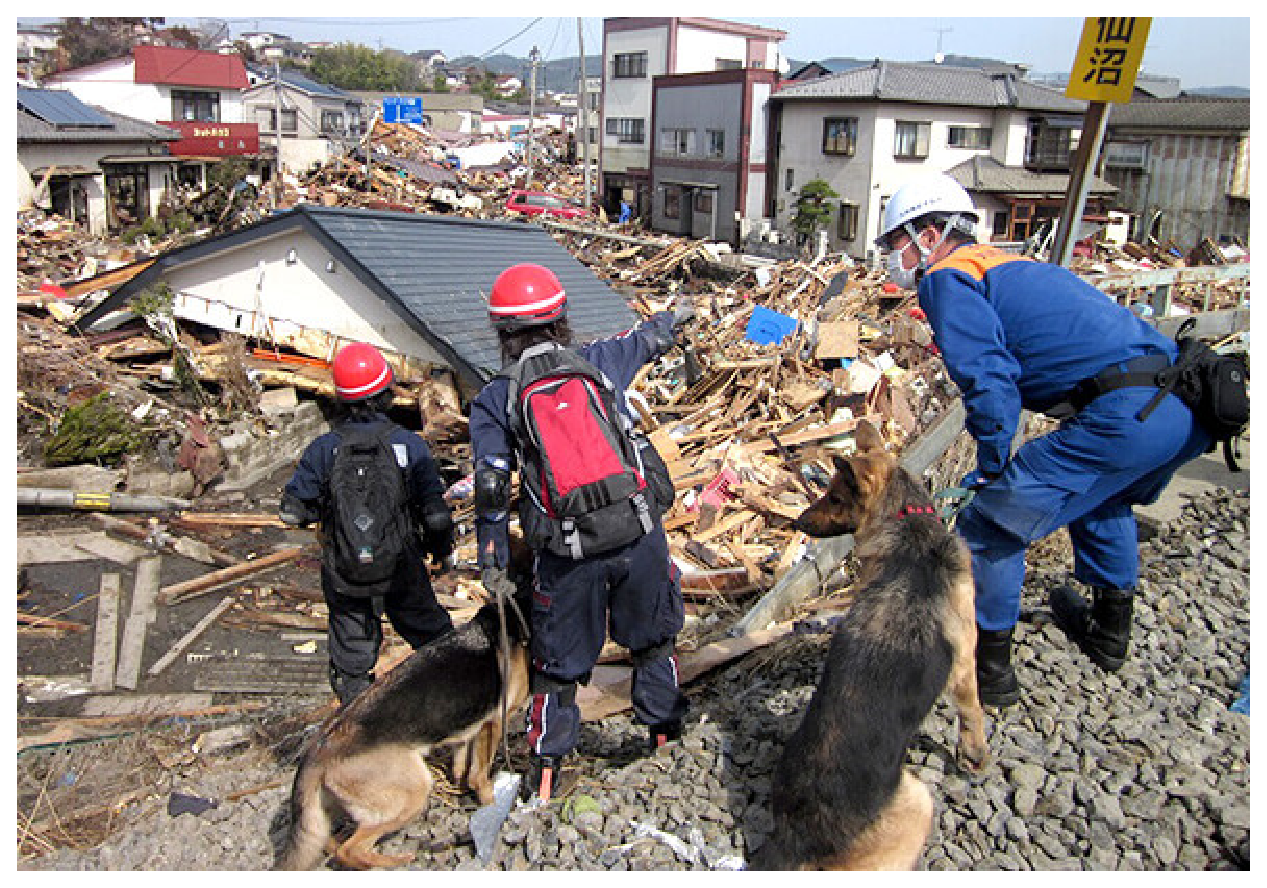
\includegraphics[width=12cm]{./Figures/resque.eps}
  \caption{被災地におけるレスキュー犬らの救助活動~\cite{buycott}より引用}
  \label{resque}
 \end{center}
\end{figure}

%%%%%%%%%%%%%%%%%%%%%%%%%%%%%%%%%%%%%%%%%%%%%%%%%%%%
%%%%%%%%%% 2章
\chapter{関連研究}
本研究では犬の一人称視点動画からの犬の活動分類を行う.人間のライフログとしての一人称動画の分類や,車載映像からの車の行動推定,第三者視点での動画分類,音声を用いた動画分類などについて紹介し,本研究との関連を述べる.

\section{タフ・ロボティクス・チャレンジ}
政府による総合科学技術・イノベーション会議が研究開発を促進している,``革新的研究開発推進プログラムImPACT''というプログラムがある~\cite{impact}.``ImPACTは研究開発を促進し,持続可能な発展性のあるイノベーションシステムの実現を目指したプログラム''であり,複数の研究開発プログラムを包括している.
タフ・ロボティクス・チャレンジはそのプラグラムのうちの一つであり,遠隔自律ロボット,屋外ロボットサービス事業の実現を目指したプログラムである.
このプログラムでは首都圏直下型地震などを想定し,刻々と変化する厳しい環境下でも実用性を保つ災害救助を目的としたロボットの研究開発が行われている.倒壊家屋や配管内を探索するロボット,悪天候でも飛行するドローンなどを用いての計測や認識,マッピング,活動支援などが達成目標として掲げられる.

\subsection{サイバー救助犬}
サイバー救助犬の研究はタフ・ロボティクス・チャレンジの一つである.災害救助用サイボーグ犬の開発を見据え,その足がかりとして研究されている.
サイバー救助犬の技術的達成目標は``救助犬の行動と状態の計測・伝送・認識・マッピング(運動・映像・声・生体信号)と制御による、救助活動支援''とされており,レスキュー犬の行動をモニタリングするために,濱田,大野らによって装着型計測・記録装置が開発された~\cite{dog01}.
図\ref{cyberdog}にレスキュー犬に装着可能な軽量な行動計測スーツ示す.これを着用したレスキュー犬はサイバー救助犬とも呼ばれる.
サイバー救助犬は各種センサを用いた計測データを記録し,リアルタイムに映像などのデータの無線配信が可能である.そのため,人の目の及ばない範囲でレスキュー犬が活動する際にもレスキュー犬の行動やその周辺環境などが把握可能である.

\begin{figure}[htbp]
 \begin{center}
  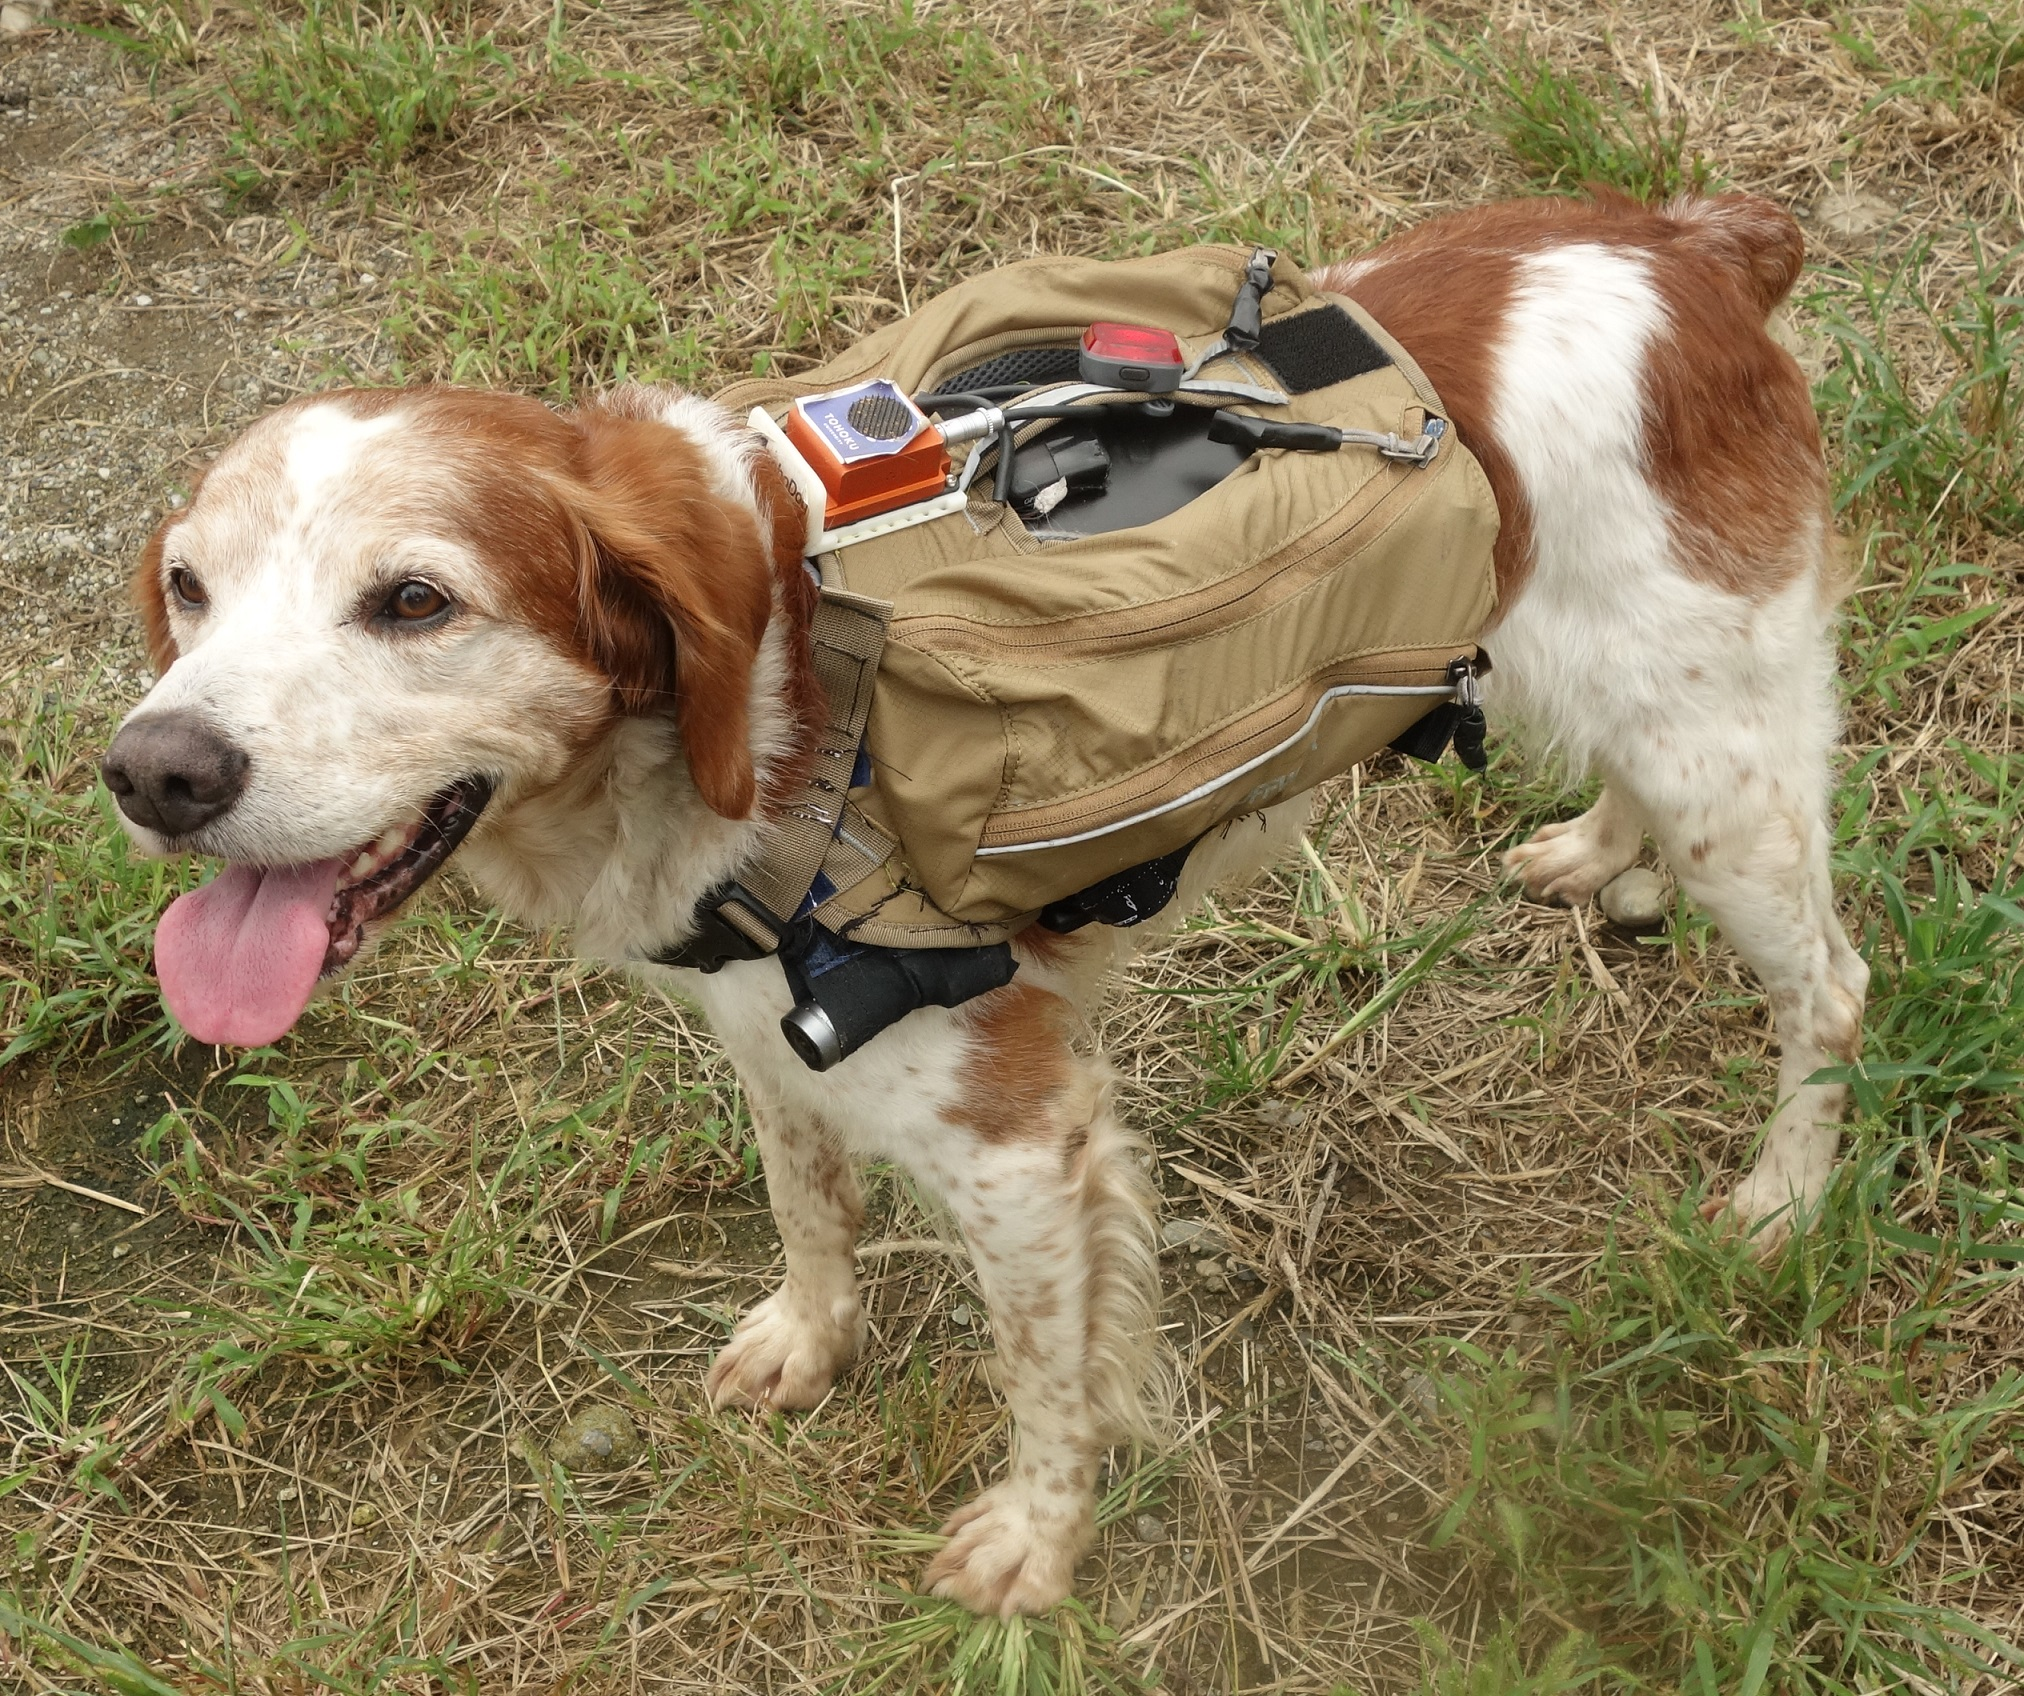
\includegraphics[width=9cm]{./Figures/cyberdog.eps}
  \caption{装着型計測・記録装置~\cite{dog01}より引用}
  \label{cyberdog}
 \end{center}
\end{figure}

\section{動画認識}
犬一人称視点映像の動きや音声の特徴は,レスキュー犬の周辺環境を知るための重要な手掛かりの1つである.
レスキュー犬の一人称動画に限らず,動画から特徴を取得してその内容を分類する類の研究は行われている.
\subsection{動作認識}
映像から動き特徴を抽出する手法は大きく分けて2つある.
1つはあらかじめ動画を複数枚の画像に分割してから特徴量を抽出する手法である.
もう1つは動画から直接特徴量を抽出する手法である.
前者は既存の画像認識の技術を簡単に流用でき,入力データが比較的小さいので学習コストが低い.
対して後者はフレーム間の情報を考慮できるが,動画を直接入力データとするため学習コストが非常に高い.
\subsubsection{Two-stream}
事前に動画から静止画を切り出してから特徴を抽出し学習する手法としてはSimonyanらによるTwo-stream convolutional networksがある~\cite{simonyan2014two}, \cite{wang2015towards}.
これは,1つの動画から通常のRGB画像とoptical flow画像を抽出し,それぞれを入力とする個々のネットワークを学習することで動き情報を考慮して動画を分類する手法である.
図~\ref{2st_network}にTwo-stream convolutionalのネットワーク構造を示す.
\begin{figure}[htbp]
 \begin{center}
  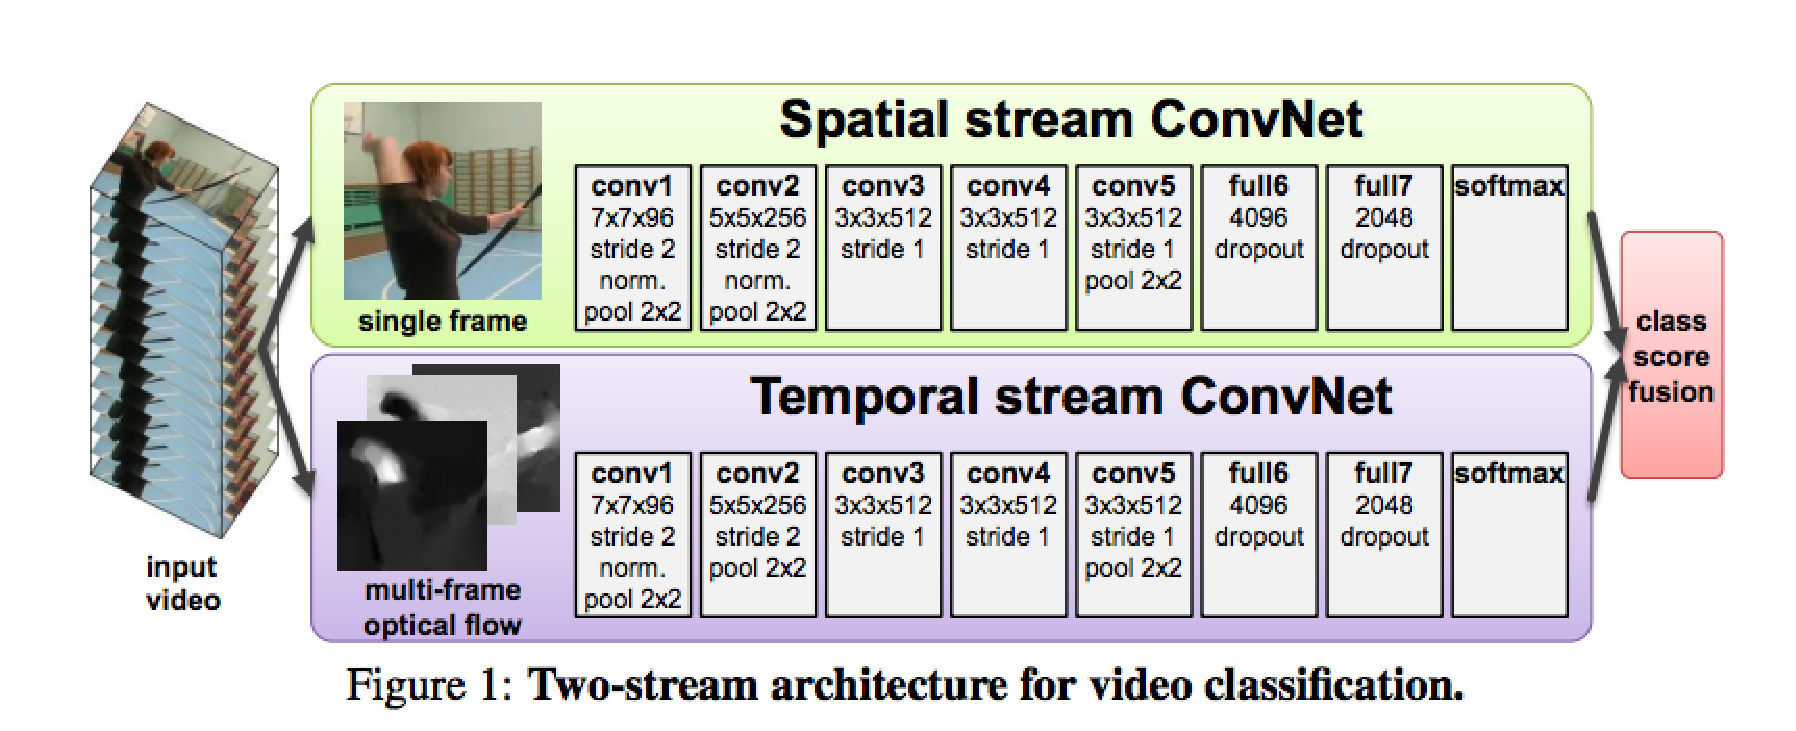
\includegraphics[width=12cm]{./Figures/two-stream.eps}
  \caption{Two-stream convolutional networks アーキテクチャ~(\cite{simonyan2014two}より引用).切り出したRGB画像とoptical flow画像を個々のネットワークに入力し、出力を合わせている.}
  \label{2st_network}
 \end{center}
\end{figure}

\subsubsection{3D Convolution}
動画から直接特徴を抽出して学習する手法としてはTranらによる3D Convolution がある~\cite{tran14}.画像に対して2次元であったフィルターを3次元形状に拡張することで,縦横の空間以外である時間方向への広がりを持って特徴抽出が可能になった.
図~\ref{3dconv_image}に3D Convolutionalの詳細を示す.
\begin{figure}[htbp]
 \begin{center}
  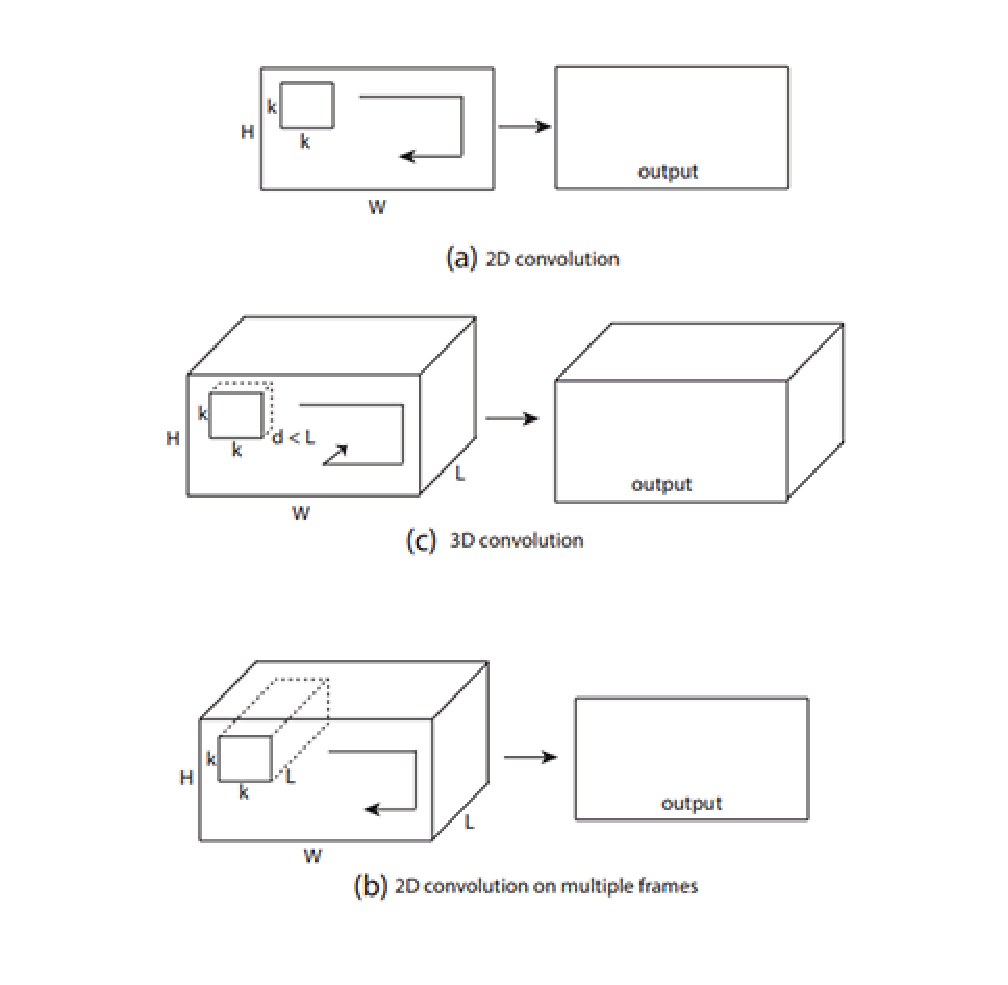
\includegraphics[width=15cm]{./Figures/3dconv.eps}
  \caption{3D Convolutionの詳細~(\cite{tran14}より引用).2D Convolutionでは縦横方向の畳み込みを行っており,3D Convolutionでは加えて時間方向への畳み込みを行っている.}
  \label{3dconv_image}
 \end{center}
\end{figure}

\subsubsection{who}

また,Ehsanらによる犬の一人称視点動画からの犬行動予測の研究がある~\cite{whoretthedog}.これは,犬の行動をモデリングし,犬が次にどのような道をたどり行動するかを予測している.

%\section{問題点}
しかし,これらの研究は犬の行動のモデリングであり,犬の周辺環境の推定などは行っていない.また,入力は動画像のみであり,音声などのデータは利用していない.レスキュー犬の課題には,犬の周辺環境情報や動画像からだけでは判断できない情報の取得が含まれている.例えばレスキュー犬は要救助者を発見するとその場で待機し吠え続けるように訓練されている.このように,動画像データからだけではなく,音声データ,および慣性データ・GPSデータなどの情報を複合的に用いてレスキュー犬の状態を判断しなければならない.本研究は動画像と音声からなるマルチモーダルな情報を入力とした犬の行動の分類を目的としている. 


\subsection{音声分類}
音声と画像から特徴を抽出する研究には以下のようなものがある.
\subsubsection{Sound Net}
音声をクラス分類する研究としてAyterらによるSound Netがある~\cite{aytar2016soundnet}.
動画から音声と画像を取り出し,画像を教師データとし,音声は生徒データとして出力が等しくなるように学習している.
図~\ref{soundnet_network}にSound Netのネットワーク構造を示す.
\begin{figure}[htbp]
 \begin{center}
  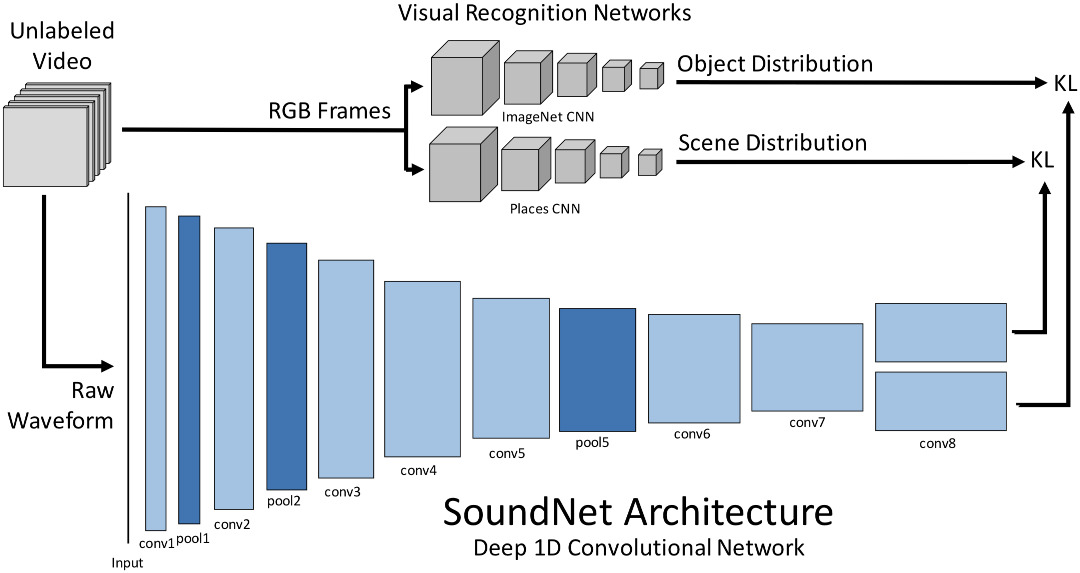
\includegraphics[width=8cm]{./Figures/soundnet.eps}
  \caption{Sound Netのアーキテクチャ~(\cite{aytar2016soundnet}より引用).動画から映像と音声を切り分け,音声に対して1次元の畳み込みを行なっている.}
  \label{soundnet_network}
 \end{center}
\end{figure}

\subsubsection{Audio-Visual Scene Analysis}
音声と動画を紐づけて,その関係を明らかにする研究としてOwensらによるAudio-Visual Scene Analysisがある~\ref{multisensory2018}.
映像内の音源特定,音声からの動作認識,複数の話者が個々の画面にいる際の話者の特定を行なっており,音声と映像の関連性を示している.
具体的な図を~\ref{audio_visual}に示す.
\begin{figure}[htbp]
 \begin{center}
  \includegraphics[width=8cm]{./Figures/audio_visual.eps}
  \caption{Audio-Visual Scene Analysis~(\cite{multisecsory2018}より引用).}
  \label{audio_visual}
 \end{center}
\end{figure}

%%%%%%%%%% 3章
\chapter{データセット}
既存の公開されている犬一人称視点動画データセットにDogCentric Actibity Dataset(DCAD)がある.
本研究ではレスキュー犬向けにラベル付けされたレスキュー犬訓練動画が必要であるため,本実験ではレスキュー犬の訓練動画を用いた.訓練動画を用いる前に,犬一人称視点動画から行動分類が可能かどうかを確認する予備実験を行なった.予備実験にはDCADを用いた.
\section{DogCentric Activity Dataset (DCAD)}
4頭の犬の背中にGoProカメラを取り付けて散歩をした動画を単一クラス分けしたデータセット.動画は320 x 240 解像度,48 frames per secondで撮影されている.散歩する地域やコースは犬毎に異なり,アノテーションはそれぞれの犬に同じラベルのアクティビティをラベル付けしている.
アクティビティは10クラス(
横断前の待機: Car, 水分の摂取: Drink, 手渡しでの食事: Feed, 左を向く: Look at left, 右を向く: Look at right, 人間が犬を撫でる: Pet, ボールで遊ぶ: Play with ball, 身体をブルブルと振る: Shake, 何かの匂いを嗅ぐ: Sniff, 歩く: Walk
)あり,それぞれ合わせて209クリップになる~\ref{DCAD labels}.
\begin{table}[tb]
  \centering{
    \caption{DogCentric Activity Dataset 内訳}\label{DCAD labels}
    \scalebox{1.00}[1.00]{
      \begin{tabler}{|r|r|r|r|r|r|r|r|r|r|}
        \hline
        Car &Drink& Feed& Left&Right& Pet & Ball&Shake&Sniff&Walk \\
        26  &   10&   25&   21&   17&   25&   14&   19&   27&   25\\
        \hline
      \end{tabler}
      }
  }
\end{table}
\section{サイバーレスキュー犬 訓練データセット}



%%%%%%%%%% 4章
\chapter{提案手法}
本研究ではレスキュー犬行動推定のために,動画像・音声のマルチラベル分類を行う.
そのため,レスキュー犬訓練データセットを認識するための手法を提案する.

入力を動画とした際に,動画から静止画像と音声を切り出し,optical flow画像を生成する.
この3つをそれぞれ別のストリームに入力し,それぞれの出力を元にレスキュー犬の行動を推定する.概念図を~\ref{easy_image}に示す.
\begin{figure}[H]
 \begin{center}
%  \includegraphics[width=10cm]{./Figures/easy_image.eps}
  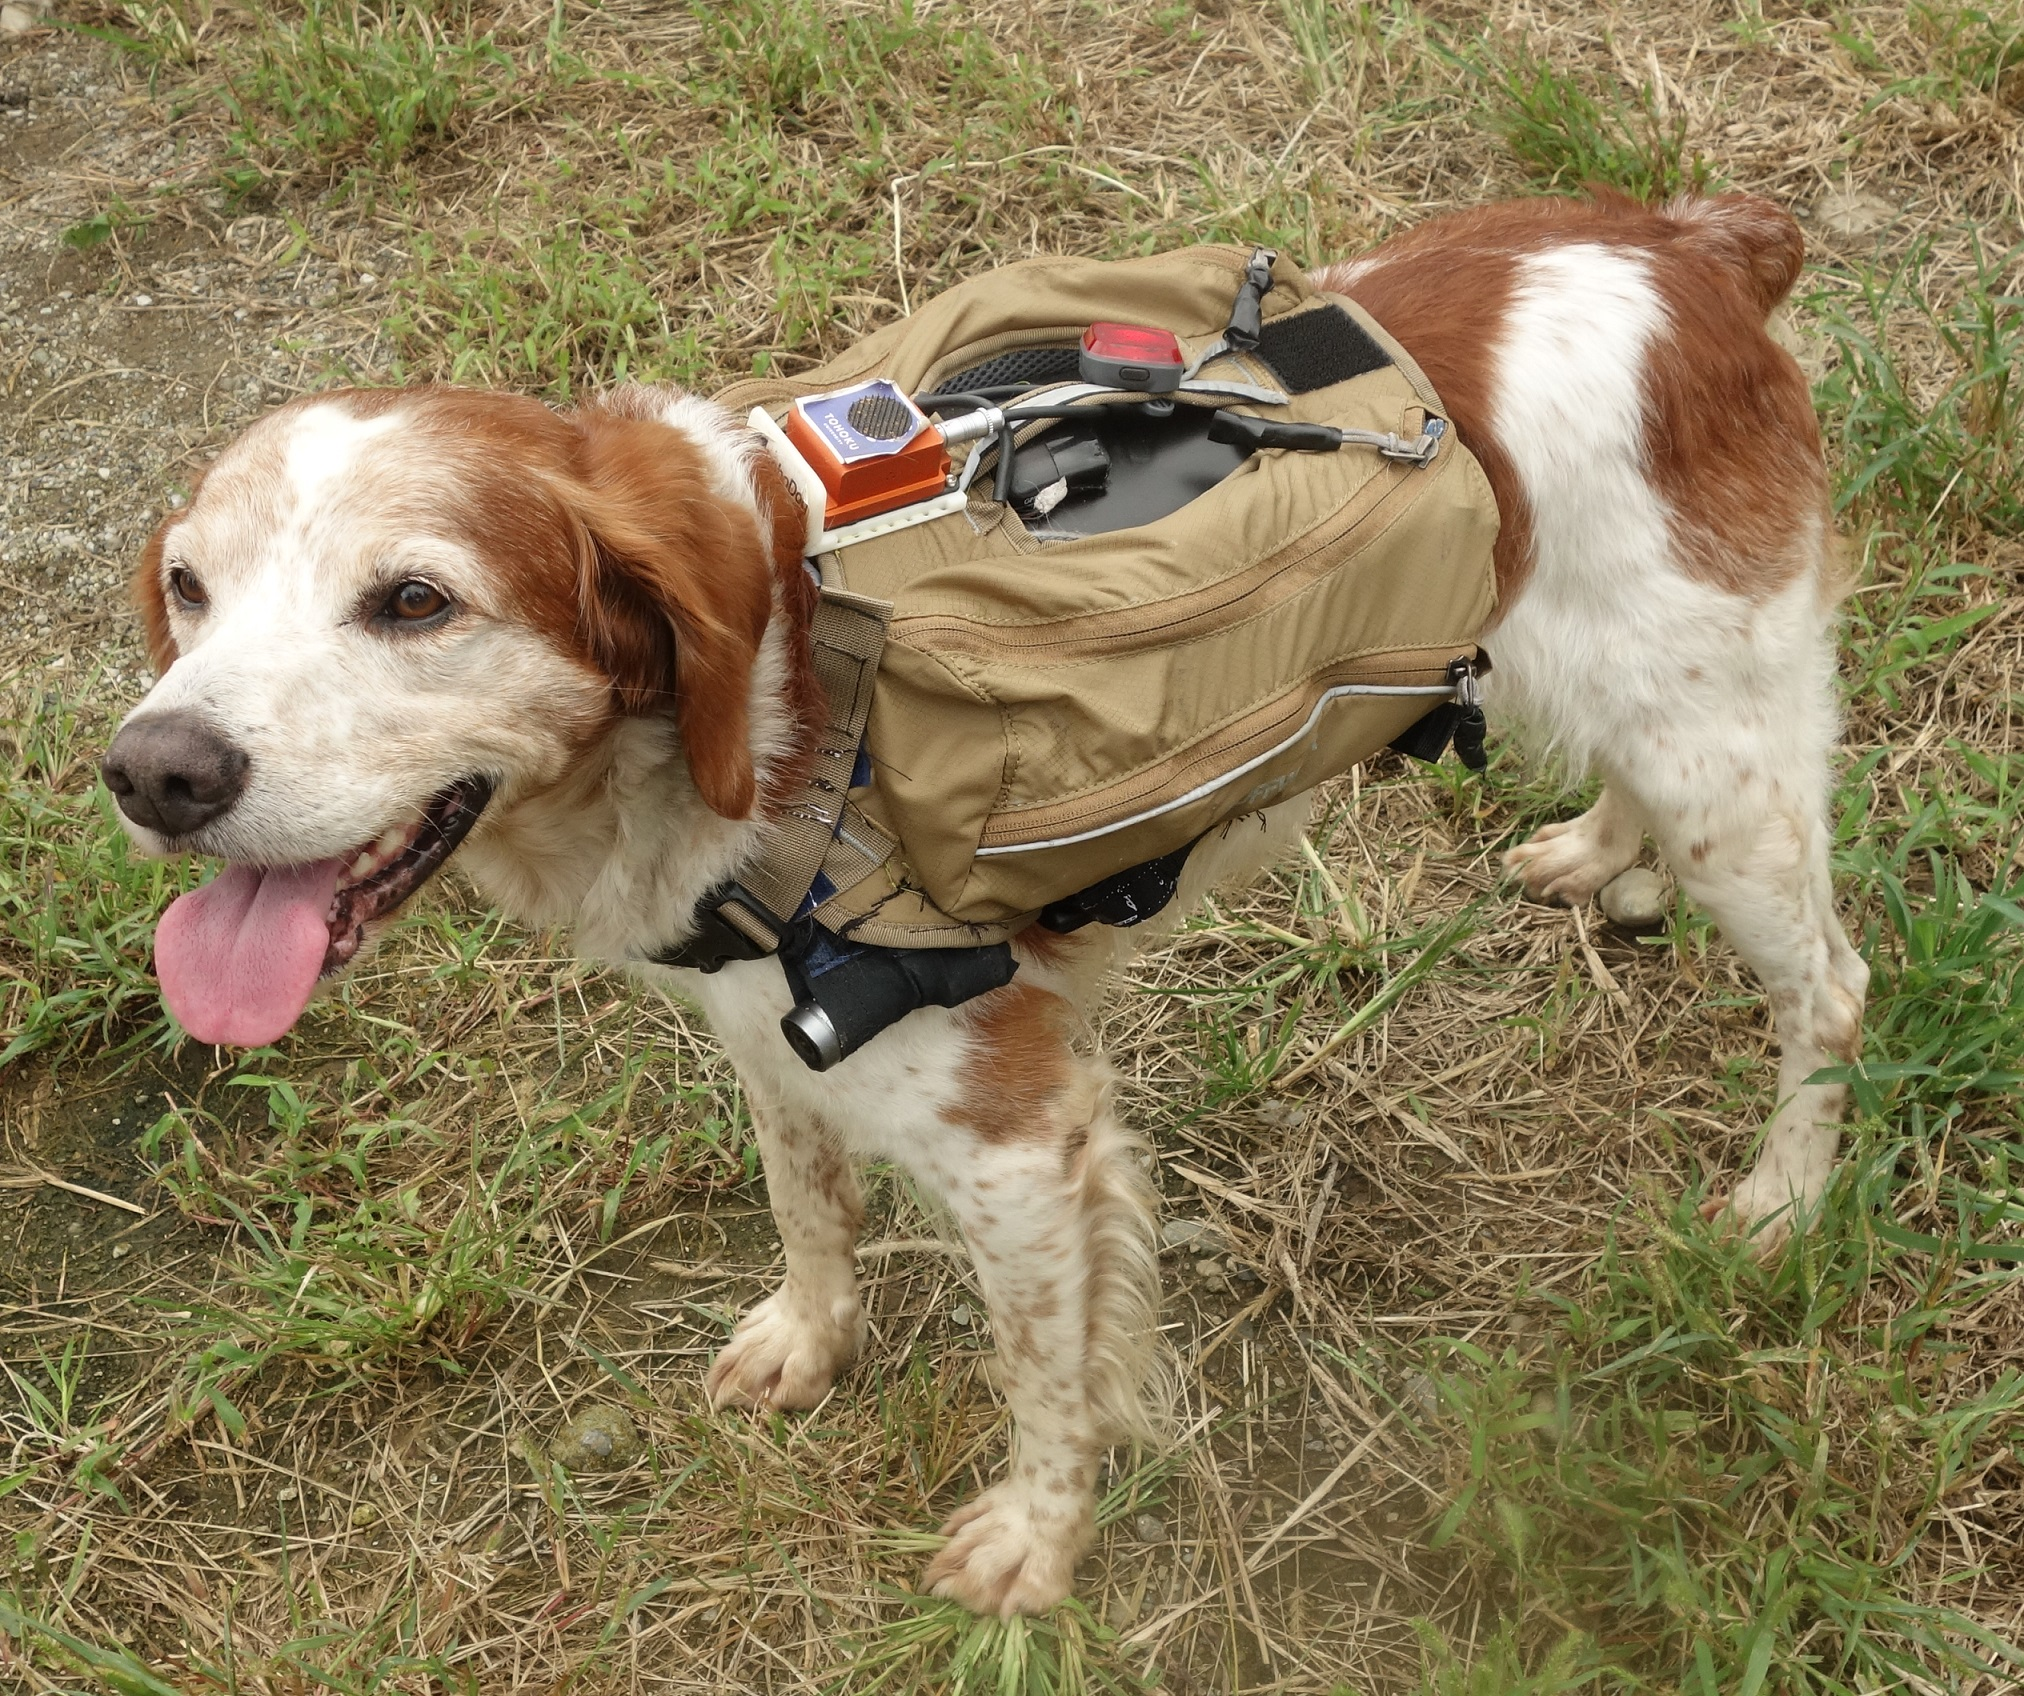
\includegraphics[width=10cm]{./Figures/cyberdog.eps}
  \caption{処理の流れの概念図を作る(提案手法の概要.入力動画から複数データを抽出し,それぞれ別のストリームへ入力する.各ストリームの出力をもとに,動画のレスキュー犬行動推定結果を最終出力とする.)}
  \label{easy_image}
 \end{center}
\end{figure}
%まず,入力となる動画から静止画像のフレーム($F_t$)を取り出し,直後の$F_{t+1}$間とのoptical flow画像($O_t$)を生成する.次に両画像から同じ構造の2つのネットワークを用いて特徴量の抽出を行う.
%そして対応する音声($A_t$)からメル周波数ケプストラム係数($M_t$)を求め,前述とは異なる構造のネットワークを用いて($M_t$)から特徴量の抽出を行う.
%最後にこれら2つあるいは3つの特徴量の組み合わせ毎に結合し,分類ネットワークでクラス分類を行う.
%この際に,音声をフレームと同じサイズで切り出すと特徴が著しく失われるため入力音声には$F_t$の前後0.5秒ずつを用いた.動画あるいは音声から実際に犬の行動を推定する場合を想定し,現実的で取り扱いやすい時間としてこれを設定した.

%分類はフレーム毎に行った.
\section{音声と画像を用いたsound/image-based Two-stream CNN}
1つ目の提案手法として,音声を用いたTwo-stream networkを提案する.
既存のTwo-stream networkを改造し,静止画と音声からの動画分類の手法である.
Two-stream networkと違い音声を用いるため,これをSound based Two-stream networkと呼称する.
Sound based Two-stream networkのアーキテクチャを図~\ref{sound-two-stream}に示す.
本研究ではこのネットワークを一般的なシングルクラス分類ではなくマルチクラス推定に用いる.
シングルクラス分類の損失関数にはCrossEntropyLossを用いてクラス確率を求めたが,マルチクラス推定にはクラス毎にSoftMarginLossを用いた.
入力を$x$,出力を$y$,クラス数を$C$とすると,マルチクラス推定の損失関数SoftMarginLossは式~\ref{softmargin}に定義される.
推定クラスが正解なら$\Sigma$内の第2項,不正解なら第1項が計算に利用するように設計されており,推定ラベルによって関数が変わる.
本研究では11クラスあり,出力yは(11)次元のバイナリとする.
閾値=0.5とし,閾値以上のクラスを推定クラスとした.
\begin{equation}
\label{softmargin}
loss(x, y) = -\frac{1}{C} * \Sigma_{i} y[i] * log((1+exp(-x[i]))^{-1}) + (1 - y[i]) * log(\frac{exp(-x[i])}{1+exp(-x[i])})
\end{equation}

学習は全てにおいて100エポック行った.学習率は1e-03~1e-06,バッチサイズは32~128の範囲で学習毎に変え制限の中で最も良い精度の結果を評価した.


\begin{figure}[htbp]
 \begin{center}
  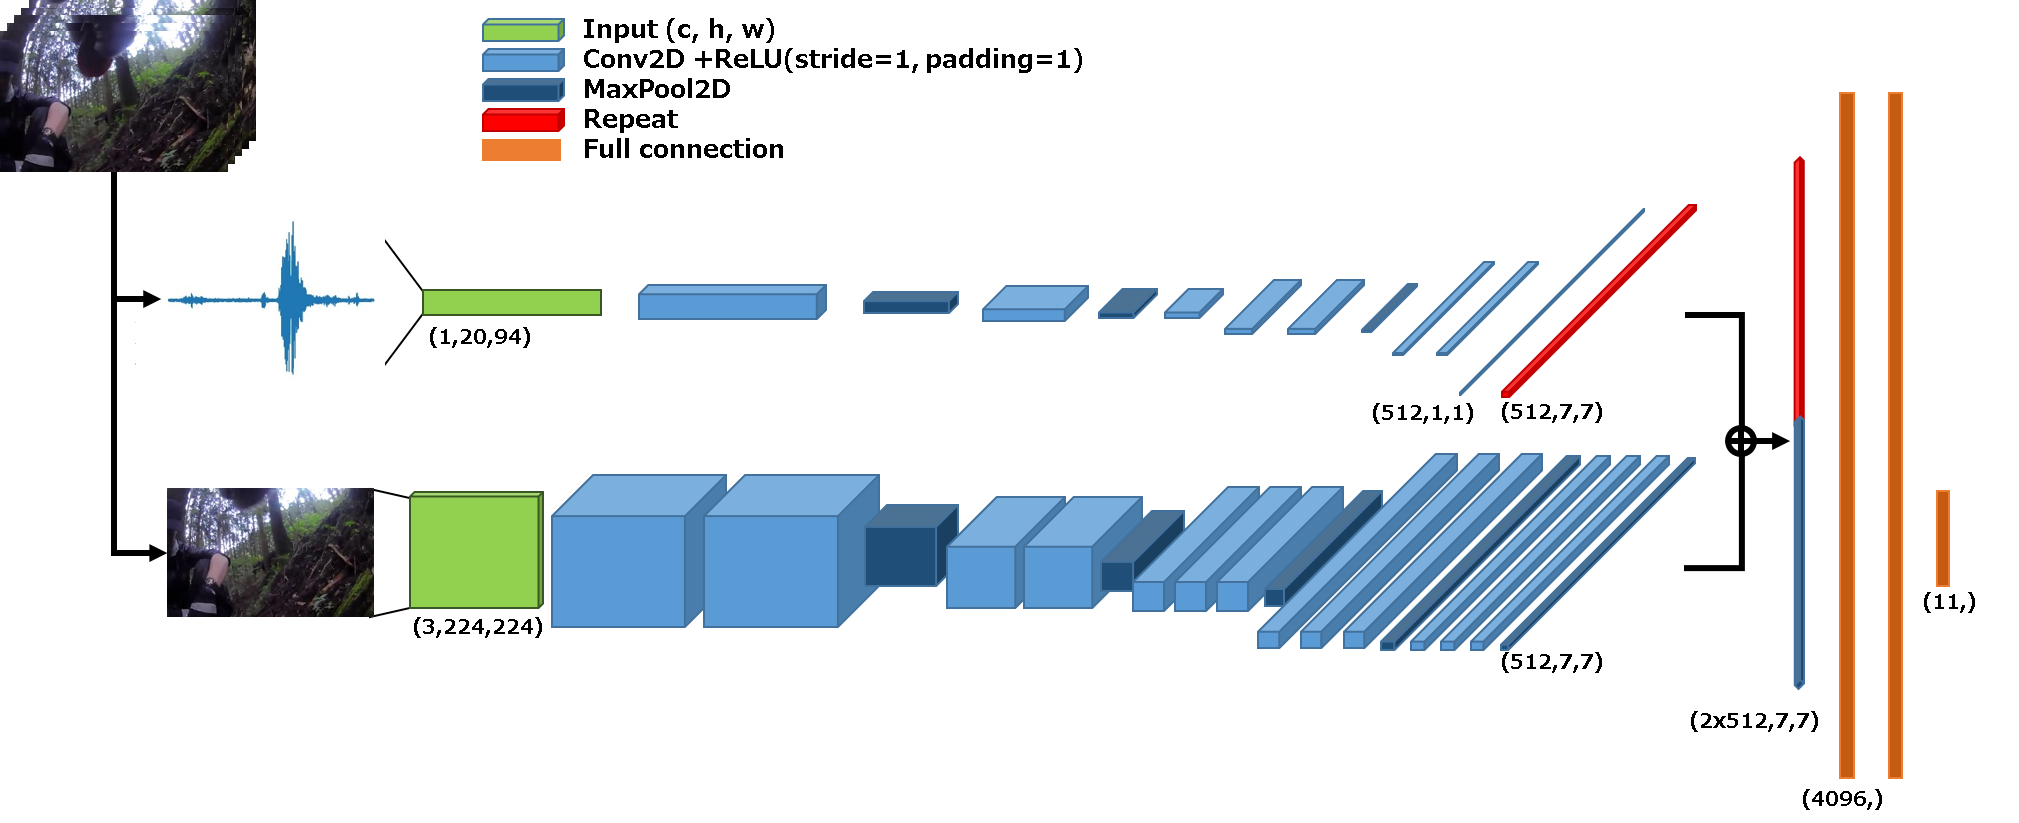
\includegraphics[width=15cm]{./Figures/soundbasedTwostream.eps}
  \caption{Sound based Two-stream (提案手法)のアーキテクチャ.(3,224,224)次元の画像と(1,20,94)次元を音声をそれぞれ別のネットワークに通し,得られた特徴を結合したのちFCレイヤを通しクラス数と同じ次元の出力を得る.}
  \label{sound-two-stream}
 \end{center}
\end{figure}



\section{音声・静止画像・optical flow画像を用いたsound/image-based Three-stream CNN}
2つ目の提案手法として,音声,静止画像,optical flow画像の3つの情報を用いたSound based Three-streamを提案する.
Sound based Two-stream networkに,画像を入力とするネットワークを加えた3つのstreamを組み合わせている.
Sound based Two-stream networkのアーキテクチャを図~\ref{sound-two-stream}に示す.
動画を31フレームとし,中央から切り出した静止画像とそれに対応する直後のoptical flow画像をそれぞれImageNetで学習済みのVGG16モデルに通し,畳み込み層の出力を結合する.
動画から切り出した音声は音声ストリームに入力する.畳み込みを繰り返すと特徴の縦横次元が小さくなるため,静止画像の畳み込みの出力と同じサイズになるように調整する.
調整は畳み込みで奥行き次元を揃えた後,同じ特徴をリピートし目的の大きさになるまでコピーして結合する.
本研究では入力音声は(1,20,94)次元の特徴に変換しており,畳み込みを繰り返して(512,1,1)次元にする.この細長い特徴を縦横に7つ並べ,(512,7,7)の特徴として静止画像とoptical flowの結合特徴に追加で結合する.

\begin{figure}[htbp]
 \begin{center}
  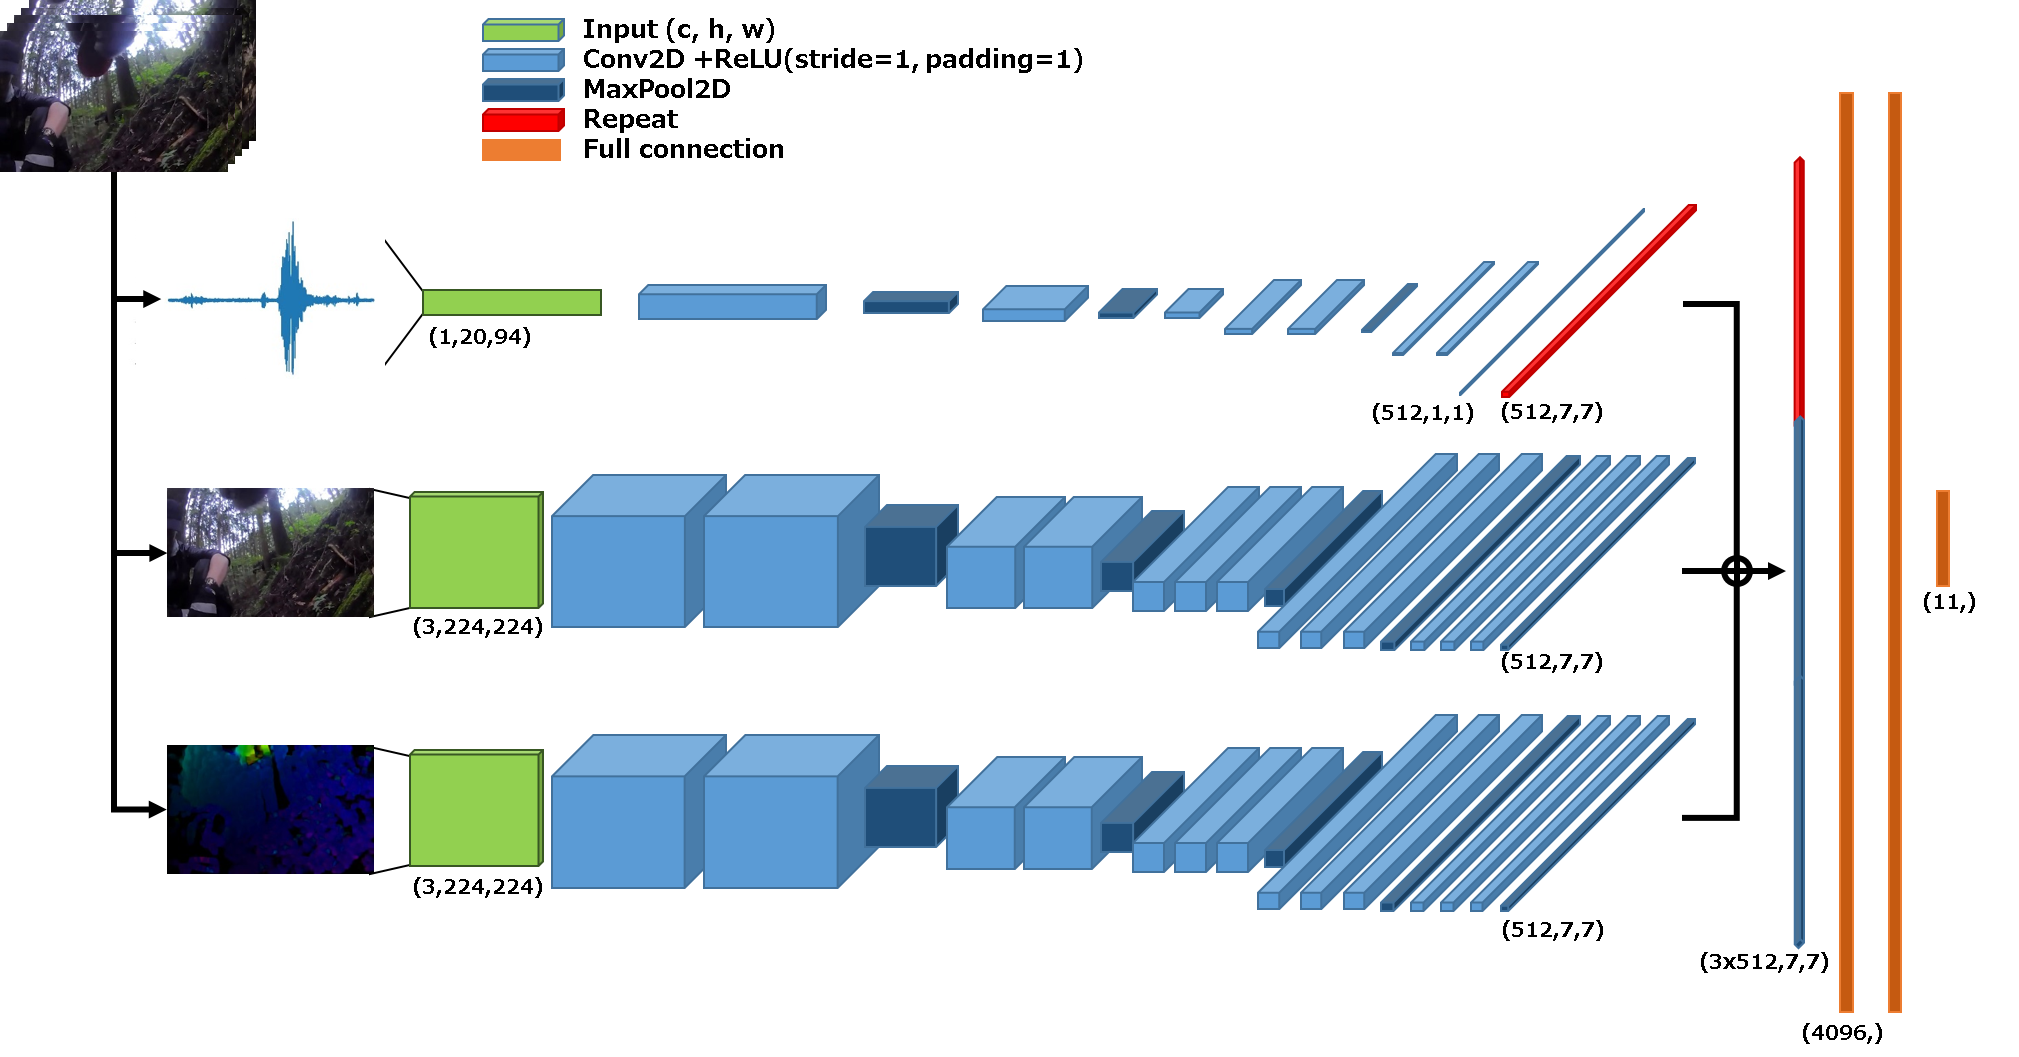
\includegraphics[width=15cm]{./Figures/soundbasedThreestream.eps}
  \caption{Sound based Three-stream (提案手法)のアーキテクチャ.(3,224,224)次元の画像と(1,20,94)次元を音声をそれぞれ別のネットワークに通し,得られた特徴を結合したのちFCレイヤを通しクラス数と同じ次元の出力を得る.}
  \label{sound-three-stream}
 \end{center}
\end{figure}

%%%%%%%%%% 5章
\chapter{実験}
予備実験を含め,行なった実験は9種類ある.

予備実験として,DCADとレスキュー犬訓練データセットの2種類のクラス分類を行なった.

本実験では,
静止画像からのマルチラベル推定,
optical flow画像からのマルチラベル推定,
音声データからのマルチラベル推定2種,
Sound based Two-stream networkを用いた音声データと静止画像からのマルチクラス推定,
同じくSound based Two-stream networkを用いた音声データとoptical flow画像からのマルチクラス推定,
そしてSound based Three-stream networkを用いた音声データと静止画像とoptical flow画像からのマルチクラス推定の7種類を行なった.
\section{予備実験:クラス分類}
DCADとレスキュー犬訓練データセットについて,それぞれクラス分類を行なった.
DCADはクリップ毎にフレーム間の平均をとり,画像として扱ってVGG16のpretrained modelを用いてfinetuningを行なった.
レスキュー犬訓練データセットは動画をラベル毎に切り出して短いクリップ群を作り,そのクリップ毎に同様にフレーム間の平均を取った画像を作成しVGG16のpretrained modelを用いてfinetuningした.
\subsection{DCAD動画像平均画像クラス分類}
予備実験の結果を~(図\ref{vgg16_res}に示す.分類率は64.3\%であった.
全般的に,データの多いクラスは精度が高い傾向にあるが,データの少ないクラスは精度が低い傾向にある.
加えて,~\(Car\)クラスは道路の進行方向に対して垂直に待機している10クラスの中で特殊なクラスであり,車などの写ったフレームの影響で分類精度が上昇していると考えられる.~\(Feed\)クラス,~\(Pet\)クラス,~\(Play\_with\_ball\)クラスは,それぞれフレーム内を人間が占める割合が多いクラスと言え,そのため混同が起こりやすいと考えられる.

\begin{figure}[htbp]
 % \begin{tabular}{cc}
 %  \begin{minipage}{0.5\textwidth}
   \begin{center}

    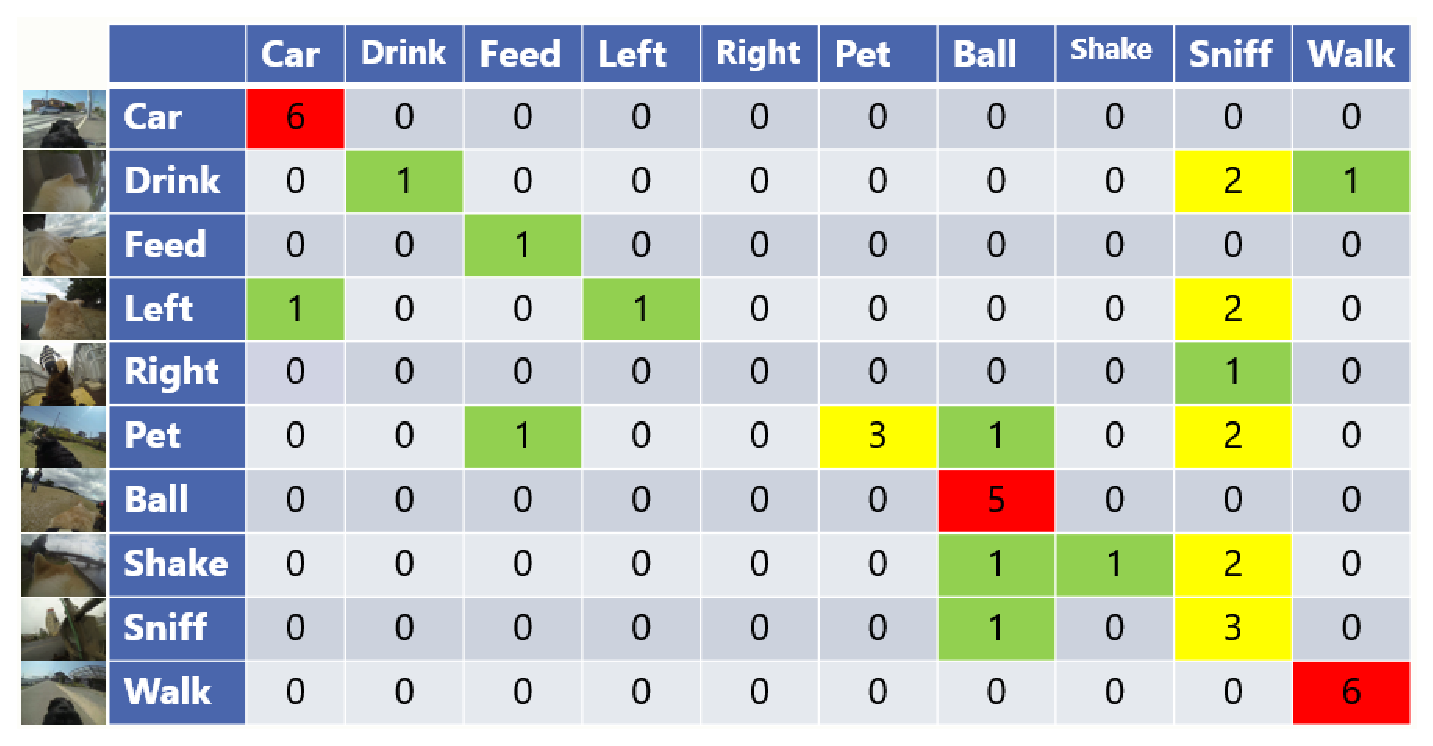
\includegraphics[scale=0.5]{./Figures/vgg16_res.eps}
    \caption{VGG16 pretrained modelとDCADによるfinetuningの結果}
    \label{vgg16_res}
   \end{center}
  % \end{minipage}
  % \begin{minipage}{0.5\textwidth}
\end{figure}

\subsection{レスキュー犬訓練データセット動画像平均画像クラス分類}
レスキュー犬訓練データセットでの予備実験の結果を図~\ref{sub_resque_res}に示す.

データ数の多いwalkクラスやstopクラスだけでなく,shakeクラスやeatクラスなどのデータ数の少ないクラスも大まかに分類できていることが分かる.
この結果によって,レスキュー犬訓練データセットからクラス分類・推定が可能であることが示された.
\begin{figure}[htbp]
  \begin{center}
    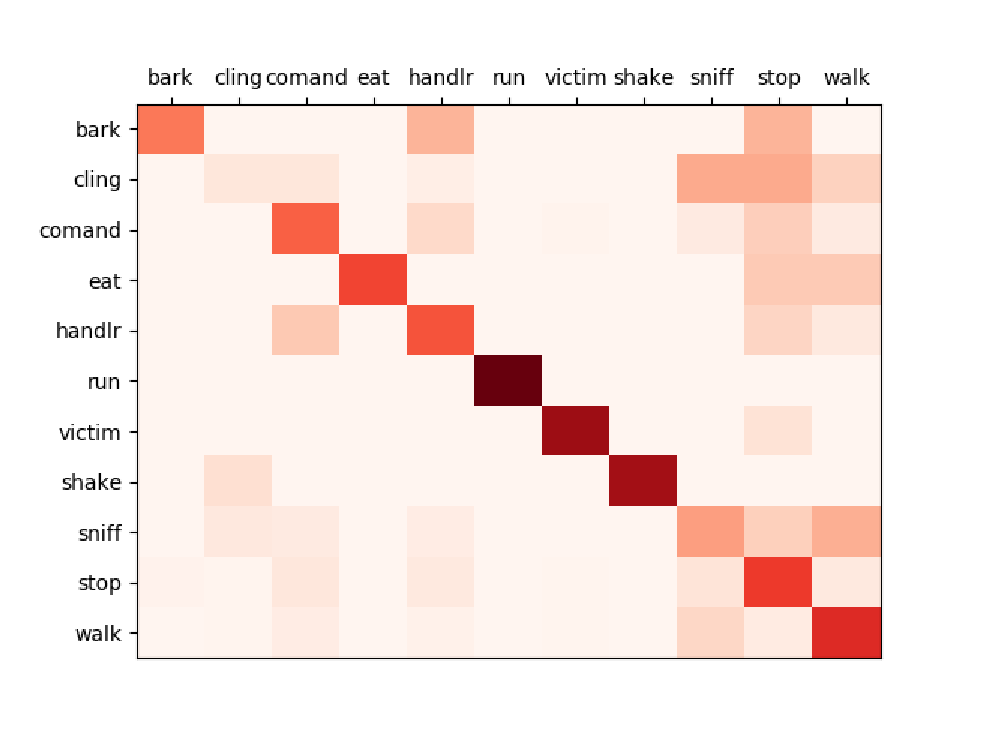
\includegraphics[scale=0.7]{./Figures/resque_mean_result.eps}
    \caption{VGG16 pretrained modelとレスキュー犬訓練データセットフレーム平均画像によるクラス分類のfinetuning結果}
    \label{sub_resque_res}
  \end{center}
\end{figure}

\subsection{オプティカルフロー動画平均画像クラス分類}
動画像のフレーム間の平均を取った手法と同様に,クリップ毎にoptical flowの平均画像を作成しVGG16のpretrained modelを用いてfinetuningを行なった.
結果を図~\ref{sub_optresque_res}に示す.

やはりデータ数の影響を受けているものの,通常の動画のフレーム平均画像とは異なる傾向が得られた.
この結果によって,optical flow画像から得られる特徴の有用性が示された.
\begin{figure}[htbp]
  \begin{center}
    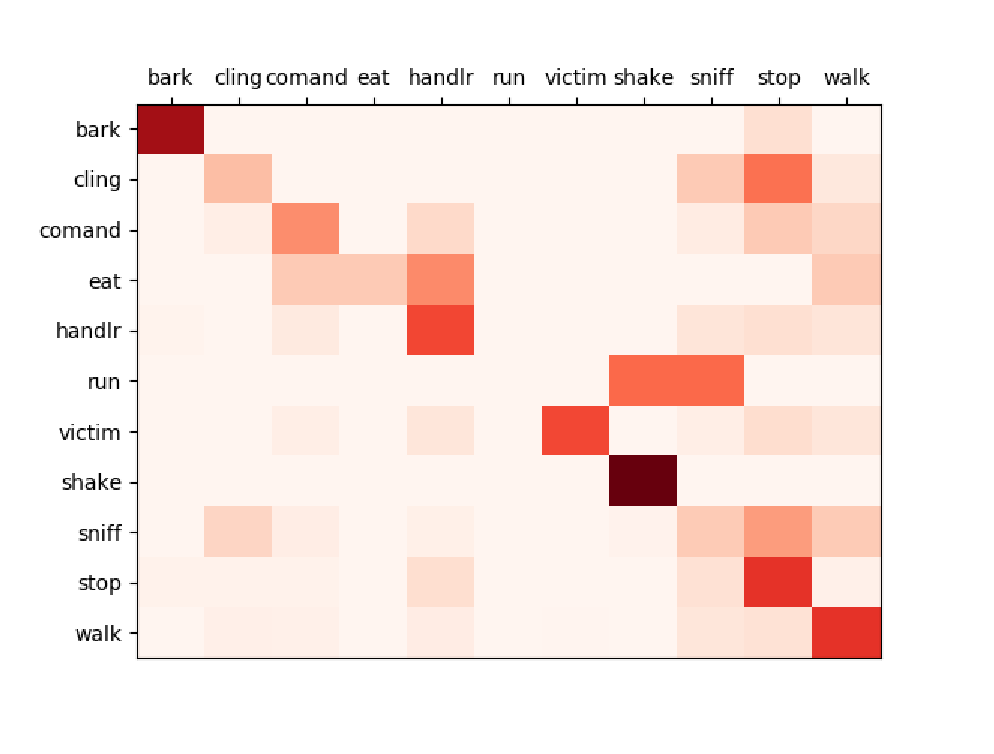
\includegraphics[scale=0.7]{./Figures/resque_optmean_result.eps}
    \caption{VGG16 pretrained modelとレスキュー犬訓練データセットoptical flow動画フレーム平均画像によるクラス分類のfinetuning結果}
    \label{sub_optresque_res}
  \end{center}
\end{figure}

%%%%%%%%%% 6章
\section{マルチラベル推定}
レスキュー犬訓練データセットのマルチラベル推定を行なった.動画で見たデータセットの前半70\%を学習、後半30\%を評価に用いた.
モデル毎にそれぞれチューニングを行い,モデル内で最も精度の良いものを示す.
各表ではクラス毎の精度と全体を合計しての精度をPrecision(適合性),Recall(再現率),Jaccard係数で示している.
なお,Jaccard係数とは\[tfrac{TP}{FP+FN+TP}\]で表され,PrecisionとRecallの両者についてF尺度と比較してより厳格な値が求まる.
レスキュー犬の行動分類にあたり,PrecisionとRecallを共に重視するためにこの係数を採用した.
よって,本研究ではJaccard係数がより大きいモデルは精度がより良いと表現する.

\subsection{静止画像からのマルチクラス推定}
静止画像からのマルチクラス推定では,ImageNetで学習したVGG16のpretrained modelを用いてのfinetuningを行なった.
推定精度を表~\ref{still_result}に示す.
%表~\ref{cyberdataset_label}と照らしあわせると,データ数の少ないものは精度が低い傾向にある.
%eatクラス,runクラスが特にその傾向を反映している.傾向とは異なるものとして,

eatクラス,runクラスが特に精度が低く,データ数の少なさと関係していると考察できる.
データ数が少ないにも関わらずPrecisionの高いshakeクラス,反対にデータ数が十分にも関わらず精度の低いsniffクラスからは,図~\ref{cyberdataset_img}に示したように画像特徴の取りやすさ、取りにくさに依存していることが確認できる.
\begin{table}[tb]
 \centering
 \caption{静止画像を用いたVGG16のfinetuning結果}\label{still_result}
 \scalebox{0.95}[1.00]{
  \begin{tabular}{|l||c|c|c|c|c|c|c|c|c|c|c|c|}
   \hline \hline
   クラス   & \rotatebox{90}{bark}& \rotatebox{90}{cling}&\rotatebox{90}{command}& \rotatebox{90}{eat}&\rotatebox{90}{handler}& \rotatebox{90}{run}&\rotatebox{90}{victim}& \rotatebox{90}{shake}& \rotatebox{90}{sniff}& \rotatebox{90}{stop}& \rotatebox{90}{walk} & \rotatebox{90}{全体}\\ \hline
%Precision & 0.626& 0.112& 0.046& 0.23& 0.249& nan& 0.347& 0.896& 0.0& 0.777& 0.602&  0.576 \\ \hline
%Recall    & 0.363& 0.227& 0.067& 0.031& 0.027& 0.0& 0.38& 0.3& 0.0& 0.704& 0.753&  0.605 \\ \hline
%Jaccard   & 0.299& 0.081& 0.028& 0.028& 0.025& 0.0& 0.222& 0.29& 0.0& 0.586& 0.503&  0.418 \\ \hline
   % seven80_6fps_still_bc-32_lr-0_sr-5_sp-30

Precision & 0.475& 0.148& 0.0& 0.377& 0.611& nan& 0.37& nan& nan& 0.74& 0.636&  0.565 \\ \hline
Recall    & 0.333& 0.108& 0.0& 0.025& 0.059& 0.0& 0.313& 0.0& 0.0& 0.742& 0.72&  0.656 \\ \hline
Jaccard   & 0.244& 0.066& 0.0& 0.024& 0.057& 0.0& 0.204& 0.0& 0.0& 0.588& 0.51&  0.436 \\ \hline
   % seven80_6fps_still_bc-32_lr-6_sr-5_sp-30
  \end{tabular}
 }
\end{table}

\subsection{optical flow画像からのマルチクラス推定}
optical flow画像からのマルチクラス推定では,静止画像からのマルチラベル推定と同じようにImageNetで学習したVGG16のpretrained modelを用いてのfinetuningを行なった.
推定精度を表~\ref{optic_result}に示す.

静止画像と比較して,shakeクラス,stopクラスなどの動き特徴の現れやすそうなクラスの精度が高くなることを期待していたが,それらを含め全体的に精度が下がった.
画像特徴が失われたため,推定が困難になった様子がうかがえる.
\begin{table}[tb]
 \centering
 \caption{optical flow画像を用いたVGG16のfinetuning結果}\label{optic_result}
 \scalebox{0.95}[1.00]{
  \begin{tabular}{|l||c|c|c|c|c|c|c|c|c|c|c|c|}
   \hline \hline
   クラス   & \rotatebox{90}{bark}& \rotatebox{90}{cling}&\rotatebox{90}{command}& \rotatebox{90}{eat}&\rotatebox{90}{handler}& \rotatebox{90}{run}&\rotatebox{90}{victim}& \rotatebox{90}{shake}& \rotatebox{90}{sniff}& \rotatebox{90}{stop}& \rotatebox{90}{walk} & \rotatebox{90}{全体}\\ \hline
%   Precision & 0.54& 0.027& 0.017& 0.183& 0.239& nan& 0.166& 0.787& 0.0& 0.761& 0.537&  0.462 \\ \hline
%   Recall    & 0.198& 0.052& 0.011& 0.007& 0.042& 0.0& 0.121& 0.185& 0.0& 0.64& 0.719&  0.578 \\ \hline
%   Jaccard   & 0.17& 0.018& 0.007& 0.007& 0.037& 0.0& 0.075& 0.176& 0.0& 0.533& 0.444&  0.345 \\ \hline
%  seven80_6fps_optic_bc-32_lr-0


   Precision & 0.265& 0.0& nan& 0.0& 0.938& nan& 0.169& nan& nan& 0.79& 0.604&  0.51 \\ \hline
   Recall    & 0.232& 0.0& 0.0& 0.0& 0.017& 0.0& 0.018& 0.0& 0.0& 0.695& 0.693&  0.664 \\ \hline
   Jaccard   & 0.141& 0.0& 0.0& 0.0& 0.017& 0.0& 0.017& 0.0& 0.0& 0.586& 0.476&  0.406 \\ \hline
   % seven80_6fps_optic_bc-32_lr-6
  \end{tabular}
 }
\end{table}

%\begin{figure}[htbp]
% \begin{center}
%  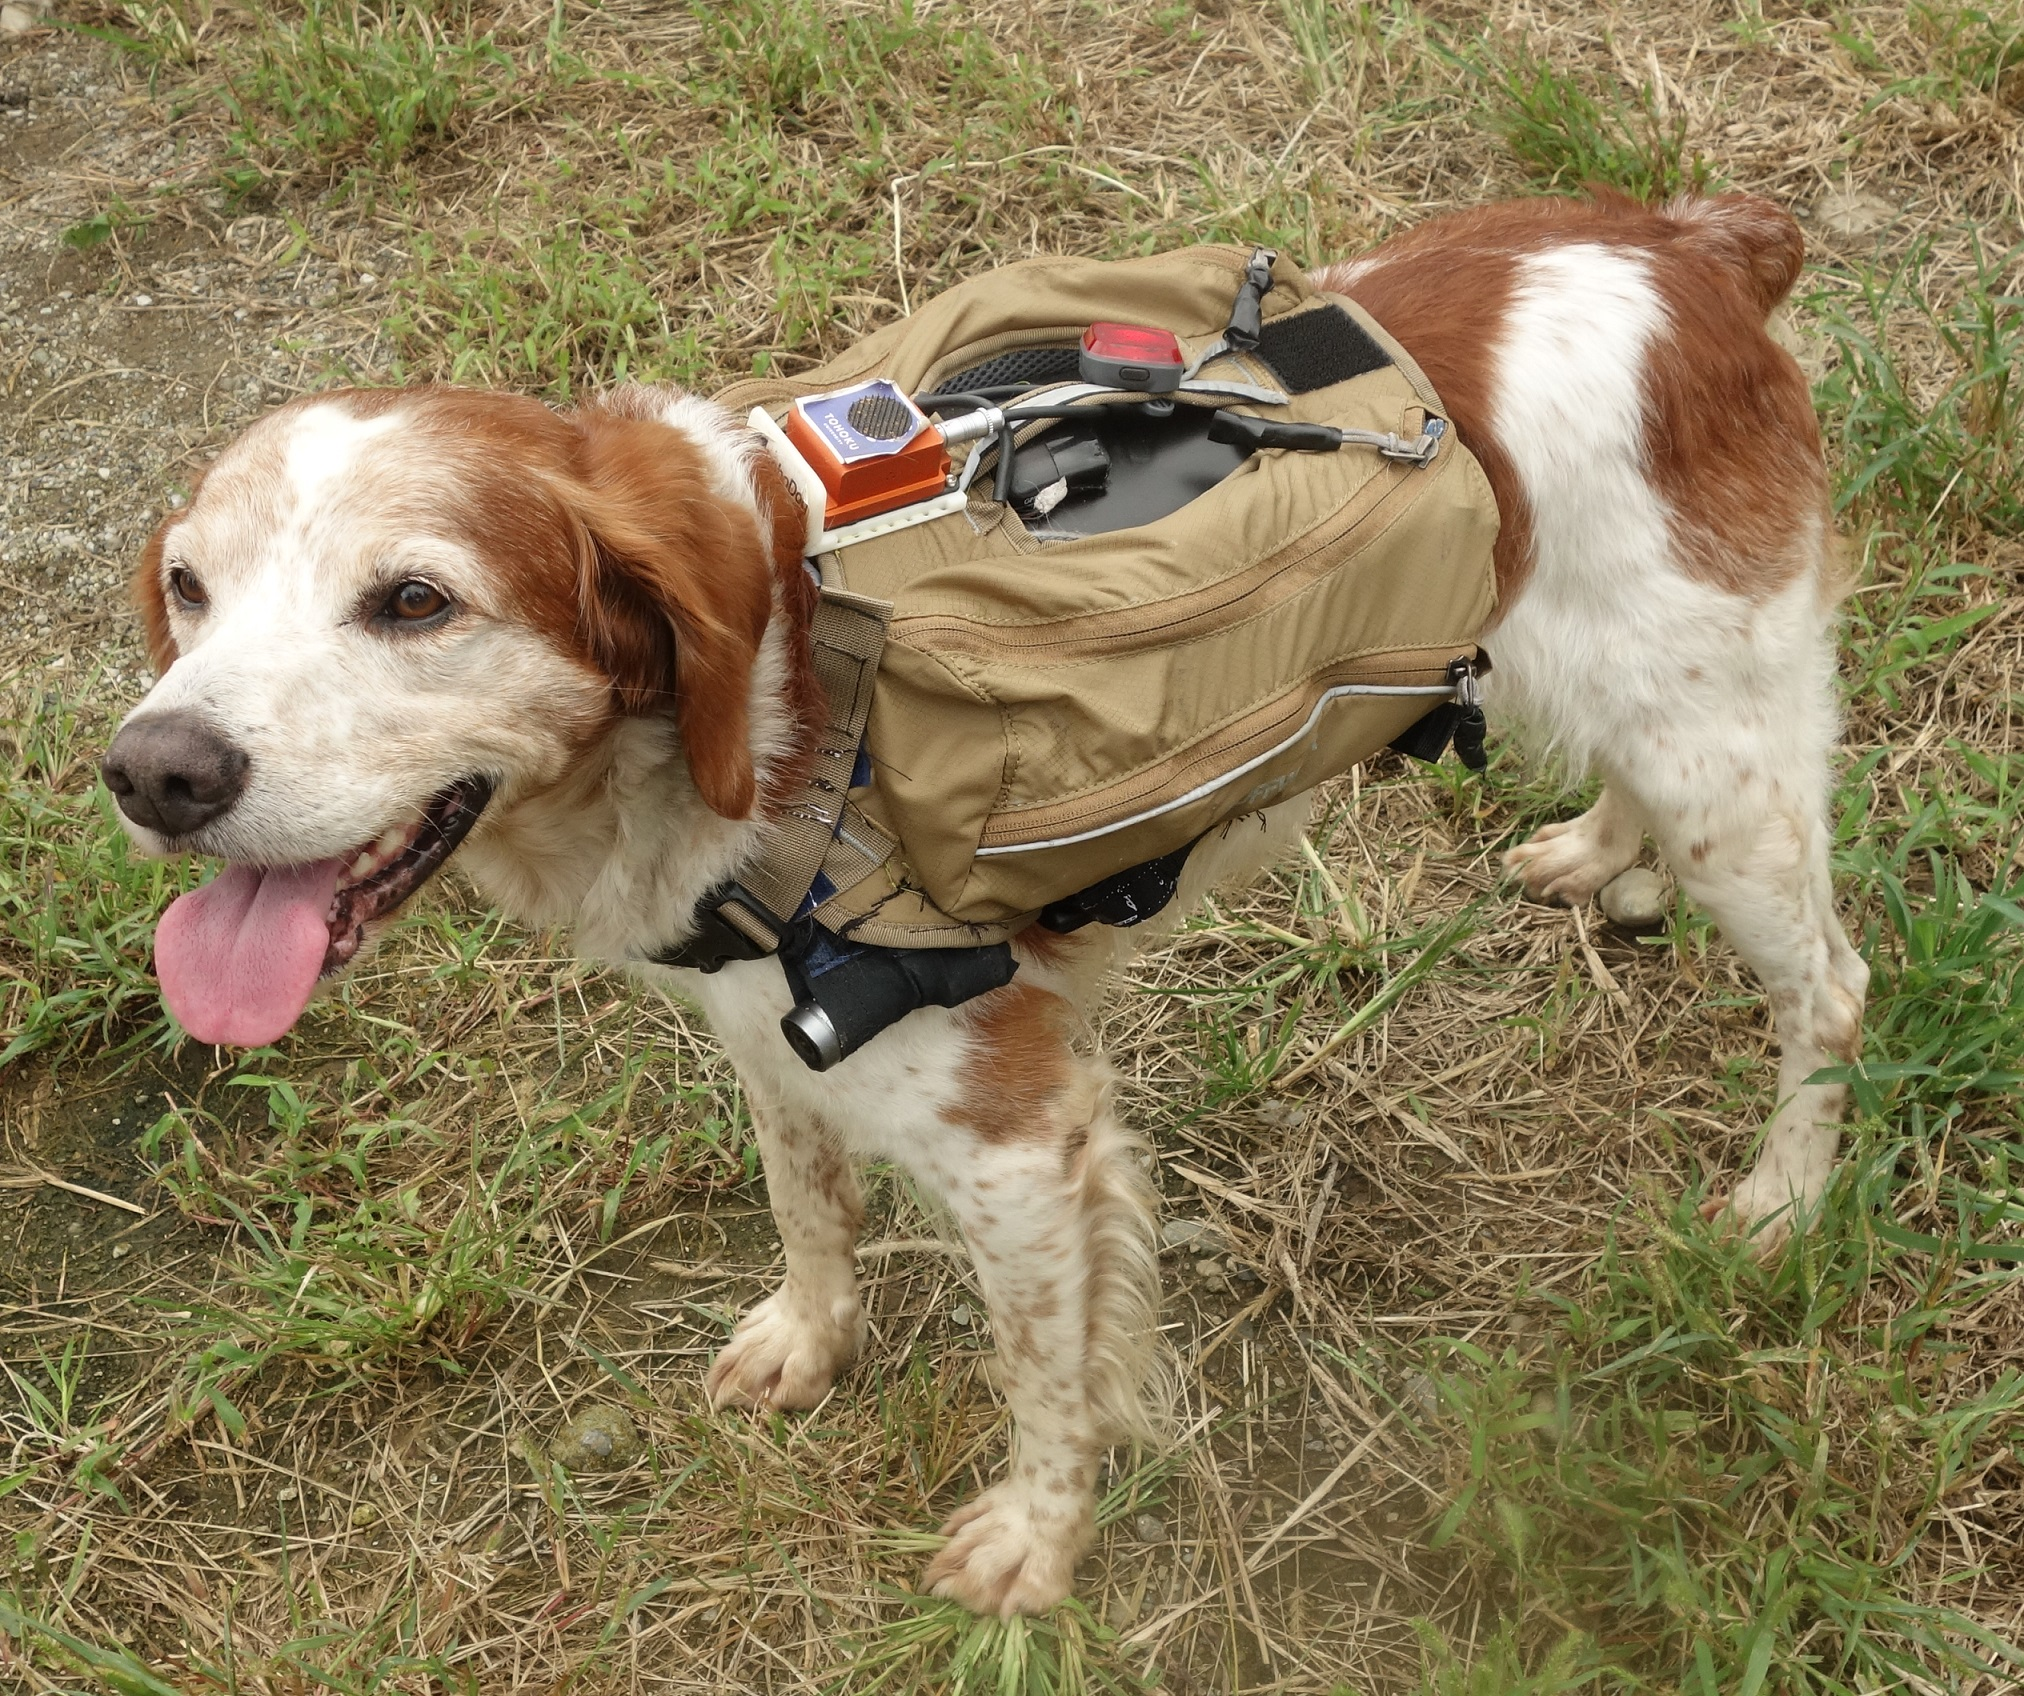
\includegraphics[width=9cm]{./Figures/cyberdog.eps}
%  \caption{装着型計測・記録装置~\cite{dog01}より引用}
%  \label{cyberdog}
% \end{center}
%\end{figure}

\subsection{音声からのマルチクラス推定}
動画の音声データのみを用いてマルチクラス推定を行なった.
ネットワークは\cite{aytar2016soundnet}の音声分類ネットワークを参考に構成した.
メル周波数スペクトラム係数を用いて音声データから特徴を取り出し,その値をネットワークへの入力とした.
29.97fpsの動画31フレーム分の音声を48000Hzとして扱い,(20, 94)次元の入力を得た.
\subsubsection{1D Convolutional network}
図~\ref{sound_network}に示したネットワークの2D Convolutionレイヤを1D Convolutionレイヤに置き換えたネットワークを用いて推定を行なった.
推定制度を表~\ref{sound_1d_result}に示す.

全体を通して,静止画像からのマルチクラス推定よりも精度が上昇した.
特に,barkクラス,commandクラス,shakeクラス,sniffクラスの精度上昇が顕著であり,音特徴がクラス推定に重要であることが示された.
\begin{table}[tb]
 \centering
 \caption{音声データを用いた1d Convolutional networkの推定結果}\label{sound_1d_result}
 \scalebox{0.95}[1.00]{
  \begin{tabular}{|l||c|c|c|c|c|c|c|c|c|c|c|c|}
   \hline \hline
   クラス   & \rotatebox{90}{bark}& \rotatebox{90}{cling}&\rotatebox{90}{command}& \rotatebox{90}{eat}&\rotatebox{90}{handler}& \rotatebox{90}{run}&\rotatebox{90}{victim}& \rotatebox{90}{shake}& \rotatebox{90}{sniff}& \rotatebox{90}{stop}& \rotatebox{90}{walk} & \rotatebox{90}{全体}\\ \hline

   %seven80_6fps_sound_bc-128_lr-4_1d
Precision & 0.909& 0.13& 0.361& 0.141& 0.245& 0.0& 0.419& 0.708& 0.583& 0.919& 0.759&  0.699 \\ \hline
Recall    & 0.717& 0.161& 0.361& 0.026& 0.24& 0.0& 0.442& 0.538& 0.781& 0.798& 0.907&  0.656 \\ \hline
Jaccard   & 0.669& 0.078& 0.22& 0.023& 0.138& 0.0& 0.274& 0.44& 0.502& 0.745& 0.704&  0.512 \\ \hline


  \end{tabular}
 }
\end{table}

\subsubsection{2D Convolutional network}
音声データから得た(20, 94)次元の入力にチャネルを追加し,(20, 94, 1)の画像としてネットワークへ入力した.
1D Convolutional networkと比較し特徴量が増え,精度がわずかに上昇した.
推定精度を表~\ref{sound_2d_label}に示す.

全体としての精度は上昇したものの,クラス別に比較した際に1D Convolutional networkで学習したモデルに劣るクラスが半数近くを占める.
学習コストなどを含めるなど評価指標を変えた際には2D Convolutional networkが劣る可能性がある.
\begin{table}[tb]
 \centering
 \caption{音声データを用いた2d Convolutional networkの推定結果}\label{sound_2d_result}
 \scalebox{0.95}[1.00]{
  \begin{tabular}{|l||c|c|c|c|c|c|c|c|c|c|c|c|}
   \hline \hline
   クラス   & \rotatebox{90}{bark}& \rotatebox{90}{cling}&\rotatebox{90}{command}& \rotatebox{90}{eat}&\rotatebox{90}{handler}& \rotatebox{90}{run}&\rotatebox{90}{victim}& \rotatebox{90}{shake}& \rotatebox{90}{sniff}& \rotatebox{90}{stop}& \rotatebox{90}{walk} & \rotatebox{90}{全体}\\ \hline
Precision & 0.844& 0.094& 0.357& 0.013& 0.192& nan& 0.407& 0.794& 0.588& 0.917& 0.808&  0.639 \\ \hline
Recall    & 0.628& 0.064& 0.285& 0.002& 0.079& 0.0& 0.284& 0.33& 0.83& 0.797& 0.898&  0.721 \\ \hline
Jaccard   & 0.563& 0.04& 0.188& 0.001& 0.059& 0.0& 0.201& 0.304& 0.524& 0.744& 0.74&  0.512 \\ \hline


   % seven80_6fps_sound_bc-64_lr-0
%Precision & 0.86& 0.116& 0.243& 0.032& 0.194& 0.0& 0.375& 0.733& 0.565& 0.909& 0.766&  0.65 \\ \hline
   %Recall & 0.754& 0.333& 0.226& 0.006& 0.128& 0.0& 0.48& 0.524& 0.824& 0.742& 0.867&  0.642 \\ \hline
   %Jaccard & 0.672& 0.094& 0.133& 0.005& 0.083& 0.0& 0.267& 0.44& 0.504& 0.691& 0.686&  0.477 \\ \hline

  \end{tabular}
 }
\end{table}

\subsection{Two-stream network}
静止画像とoptical flow画像を学習していないVGG16ネットワークにそれぞれ入力し,得られた2つの出力を結合した結果からマルチクラス推定を行なった.
推定結果を表~\ref{stilloptic_result}に示す.

静止画像単体,optical flow画像単体からの推定と比較して精度がわずかに上昇している.
特にsniffクラスなどが劇的に精度が上昇している.動画から得られた静止画像の画像特徴に加えて,optical flowから得られる動き特徴をそれぞれ用いた学習ができていると考えられる.
ただし,shakeクラスなど,静止画像とoptical flow画像がお互いに悪影響を与え全く分類できなくなってしまったクラスも存在している.
\begin{table}[tb]
 \centering
 \caption{Two-stream networkの推定結果}\label{stilloptic_result}
 \scalebox{0.95}[1.00]{
  \begin{tabular}{|l||c|c|c|c|c|c|c|c|c|c|c|c|}
   \hline \hline
   クラス   & \rotatebox{90}{bark}& \rotatebox{90}{cling}&\rotatebox{90}{command}& \rotatebox{90}{eat}&\rotatebox{90}{handler}& \rotatebox{90}{run}&\rotatebox{90}{victim}& \rotatebox{90}{shake}& \rotatebox{90}{sniff}& \rotatebox{90}{stop}& \rotatebox{90}{walk} & \rotatebox{90}{全体}\\ \hline
Precision & 0.522& 0.04& 0.315& 0.0& 0.395& nan& 0.478& nan& 0.472& 0.848& 0.771&  0.571 \\ \hline
Recall    & 0.122& 0.033& 0.047& 0.0& 0.204& 0.0& 0.36& 0.0& 0.813& 0.807& 0.833&  0.646 \\ \hline
Jaccard   & 0.11& 0.018& 0.043& 0.0& 0.155& 0.0& 0.259& 0.0& 0.426& 0.705& 0.668&  0.435 \\ \hline

   % seven80_6fps_stilloptic_bc-128_lr-0_sr-5_sp-20

  \end{tabular}
 }
\end{table}

\subsection{Sound based Two-stream network}
音声データに静止画像,optical flow画像を個別に組み合わせ,マルチクラス推定を行なった.
音声の特徴を取り出すネットワークには2D Convolutional networkを用いた.
\subsubsection{音声データと静止画像からのマルチクラス推定}
音声と静止画像を組み合わせたマルチクラス推定の結果を表~\ref{stillsound_result}に示す.
\begin{table}[tb]
 \centering
 \caption{音声と静止画像からのマルチクラス推定結果}\label{stillsound_result}
 \scalebox{0.95}[1.00]{
  \begin{tabular}{|l||c|c|c|c|c|c|c|c|c|c|c|c|}
   \hline \hline
   クラス   & \rotatebox{90}{bark}& \rotatebox{90}{cling}&\rotatebox{90}{command}& \rotatebox{90}{eat}&\rotatebox{90}{handler}& \rotatebox{90}{run}&\rotatebox{90}{victim}& \rotatebox{90}{shake}& \rotatebox{90}{sniff}& \rotatebox{90}{stop}& \rotatebox{90}{walk} & \rotatebox{90}{全体}\\ \hline
  Precision & 0.909& 0.05& 0.312& 0.051& 0.249& 0.042& 0.42& 0.56& 0.592& 0.885& 0.787&  0.661 \\ \hline
Recall    & 0.709& 0.077& 0.341& 0.028& 0.177& 0.002& 0.537& 0.589& 0.758& 0.802& 0.855&  0.673 \\ \hline
Jaccard   & 0.662& 0.031& 0.195& 0.018& 0.115& 0.002& 0.308& 0.402& 0.498& 0.726& 0.694&  0.5 \\ \hline


   %seven80_6fps_stillsound_bc-32_lr-05
  \end{tabular}
 }
\end{table}

\subsubsection{音声データとoptidcal flow画像からのマルチクラス推定}
音声とoptical flow画像を組み合わせたマルチクラス推定の結果を表~\ref{opticsound_result}に示す.
\begin{table}[tb]
 \centering
 \caption{音声とoptical flow画像からのマルチクラス推定結果}\label{opticsound_result}
 \scalebox{0.95}[1.00]{
  \begin{tabular}{|l||c|c|c|c|c|c|c|c|c|c|c|c|}
   \hline \hline
   クラス   & \rotatebox{90}{bark}& \rotatebox{90}{cling}&\rotatebox{90}{command}& \rotatebox{90}{eat}&\rotatebox{90}{handler}& \rotatebox{90}{run}&\rotatebox{90}{victim}& \rotatebox{90}{shake}& \rotatebox{90}{sniff}& \rotatebox{90}{stop}& \rotatebox{90}{walk} & \rotatebox{90}{全体}\\ \hline
Precision & 0.887& 0.071& 0.332& 0.052& 0.245& 0.143& 0.329& 0.692& 0.564& 0.881& 0.791&  0.681 \\ \hline
Recall    & 0.729& 0.177& 0.441& 0.019& 0.198& 0.01& 0.409& 0.424& 0.782& 0.845& 0.847&  0.641 \\ \hline
Jaccard   & 0.667& 0.054& 0.234& 0.014& 0.123& 0.01& 0.223& 0.356& 0.487& 0.759& 0.692&  0.493 \\ \hline

%seven80_6fps_opticsound_bc-64_lr-0
  \end{tabular}
 }
\end{table}

\subsection{Sound based Three-stream network}
表~\ref{stillopticsound_result}に示す.
\begin{table}[tb]
 \centering
 \caption{still optic sound}\label{stillopticsound_result}
 \scalebox{0.95}[1.00]{
  \begin{tabular}{|l||c|c|c|c|c|c|c|c|c|c|c|c|}
   \hline \hline
   クラス   & \rotatebox{90}{bark}& \rotatebox{90}{cling}&\rotatebox{90}{command}& \rotatebox{90}{eat}&\rotatebox{90}{handler}& \rotatebox{90}{run}&\rotatebox{90}{victim}& \rotatebox{90}{shake}& \rotatebox{90}{sniff}& \rotatebox{90}{stop}& \rotatebox{90}{walk} & \rotatebox{90}{全体}\\ \hline
Precision & 0.888& 0.165& 0.282& 0.188& 0.313& 0.212& 0.527& 0.708& 0.621& 0.891& 0.822&  0.702 \\ \hline
Recall    & 0.623& 0.423& 0.355& 0.092& 0.306& 0.029& 0.709& 0.492& 0.783& 0.861& 0.86&  0.663 \\ \hline
Jaccard   & 0.577& 0.135& 0.186& 0.066& 0.183& 0.026& 0.433& 0.409& 0.53& 0.779& 0.725&  0.518 \\ \hline


%seven80_6fps_stillopticsound_bc-128_lr-0
  \end{tabular}
 }
\end{table}

%%%%%%%%%% 7章
%\section{考察}
全体の結果を表~\ref{expetiments_result}に示す.



\begin{table}[tb]
 \centering
 \caption{各実験比較表}\label{expetiments_result}
 \scalebox{0.80}[0.80]{
  \begin{tabular}{|l||c|c|c|c|c|c|c|c|c|c|c|c|}
   \hline \hline
   & \rotatebox{90}{bark}& \rotatebox{90}{cling}&\rotatebox{90}{command}& \rotatebox{90}{eat}&\rotatebox{90}{handler}& \rotatebox{90}{run}&\rotatebox{90}{victim}& \rotatebox{90}{shake}& \rotatebox{90}{sniff}& \rotatebox{90}{stop}& \rotatebox{90}{walk} & \rotatebox{90}{全体}\\ \hline
静止画像   & 0.244& 0.066& 0.0& 0.024& 0.057& 0.0& 0.204& 0.0& 0.0& 0.588& 0.51&  0.436 \\ \hline
optical flow   & 0.141& 0.0& 0.0& 0.0& 0.017& 0.0& 0.017& 0.0& 0.0& 0.586& 0.476&  0.406 \\ \hline
音声 (Conv1D)   & {\bf 0.669}& 0.078& 0.22& 0.023& 0.138& 0.0& 0.274& {\bf 0.44}& 0.502& 0.745& 0.704&  0.512 \\ \hline
音声 (Conv2D)   & 0.563& 0.04& 0.188& 0.001& 0.059& 0.0& 0.201& 0.304& 0.524& 0.744& 0.74&  0.512 \\ \hline
静止画像+optical   & 0.11& 0.018& 0.043& 0.0& 0.155& 0.0& 0.259& 0.0& 0.426& 0.705& 0.668&  0.435 \\ \hline
静止画像+音声   & 0.662& 0.031& 0.195& 0.018& 0.115& 0.002& 0.308& 0.402& 0.498& 0.726& 0.694&  0.5 \\ \hline
optical flow+音声   & 0.667& 0.054& {\bf 0.234}& 0.014& 0.123& 0.01& 0.223& 0.356& 0.487& 0.759& 0.692&  0.493 \\ \hline
静止+optical+音声   & 0.577& {\bf 0.135}& 0.186& {\bf 0.066}& {\bf 0.183}& {\bf 0.026}& {\bf 0.433}& 0.409& {\bf 0.53}& {\bf 0.779}& {\bf 0.725}& {\bf 0.518} \\ \hline
  \end{tabular}
 }
\end{table}




\chapter{まとめ,今後の課題}
Sound based Three-streamの提案と,提案手法を用いたレスキュー犬の行動推定を行なった.
提案手法との比較のために行なった実験は以下である.
\begin{itemize}
  \item 静止画像からの犬行動マルチラベル推定
  \item optical flow画像からの犬行動マルチラベル推定
  \item 音声からの犬行動マルチラベル推定
  \item 静止画像とoptical flow画像からの犬行動マルチラベル推定
  \item 音声と静止画像からの犬行動マルチラベル推定
  \item 音声とoptical flow画像からの犬行動マルチラベル推定
  \item 音声と静止画とoptical flow画像からの犬行動マルチラベル推定
\end{itemize}
結果は提案手法が最も高く,音声・静止画像・optical flow画像のそれぞれに必要な情報が含まれており,3つのデータにそれぞれ必要な情報が含まれているとわかった.
精度は51.2\%と数値では決して高いとは言えないが,約30fpsの動画で1/5フレーム毎に行なった推定の結果であるため非実用的とも言えない結果となった.

今回は研究の範囲としなかったが,レスキュー犬行動動画の入力に対してリアルタイムに結果を出すことも求められる.
また,実験に対する疑問として音声フレームの長さはどの程度か適しているのか判断できていない.
これの変更でどの程度影響があるのかを検証し,より適切な音声フレーム長が判断できればより高い精度も期待できる.

%{\scriptsize % 7pt
%{\footnotesize % 8pt
%{\small % 9pt
%\bibliographystyle{ieee}
\bibliographystyle{junsrt}
\bibliography{ref}
%}
% \begin{footnotesize}
% %{\small
% \bibliography{ref}
% \bibliographystyle{junsrt}
% %}
% \end{footnotesize}
\end{document}


%%%%%%%%%% 目次に参考文献を加える
\addcontentsline{toc}{chapter}{参考文献}
%%%%%%%%%% 参考文献
\bibliographystyle{junsrt}
\bibliography{bib}

%付録があればここで書く
%%%%%%%%%% 付録A
%%%%%%%%%% 付録B
%\input{}

%%%%%

\end{document}
